\chapter{Improving Model Performance with additional Health Data}
\label{cha:resultsaddFeatures}

To improve the accuracy and robustness of our health data analysis, this chapter focuses on integrating additional health metrics into the dataset. In chapter ~\ref{cha:results}, we primarily worked with data measured by the Apple Watch Ultra, excluding some crucial information from the study protocols. Now, we aim to enhance our analysis by incorporating all available data, including those from study protocols and additional Apple Watch Ultra measurements. This comprehensive approach will allow us to evaluate how these extra features impact the performance of our predictive models and provide a deeper understanding of health trends and risk factors.

\section{Additional Data Features}

In this part of the work, we focus on integrating the 6MWT documentation for each subject. During this process, we discovered significant discrepancies in the distance measurements recorded by the Apple Watch Ultra. 

\subsection{Additional Distance Data}

Initially, we calculated the real distance by multiplying the leg length by the number of steps taken, where the 'Steps' column represents the difference between the 'Steps (before)' and 'Steps (after)' columns. This resulted in three different distance metrics: 'Calculated m', 'Distance (km)' and 'real\_Distance'.
The term 'leg length' encompasses the distance from the heel to the inner pubic bone (as detailed in the study protocol). All columns related to steps were published in the shared table. The 'Calculated m' values were also entered into the shared table and the values 'Distance (km)' was measured using the Apple Watch Ultra, and the 'real distance' was computed manually, as explained in the text. 
These metrics were then plotted for visual comparison to evaluate the discrepancies.

\FloatBarrier
\begin{figure}[h!]
    \centering
    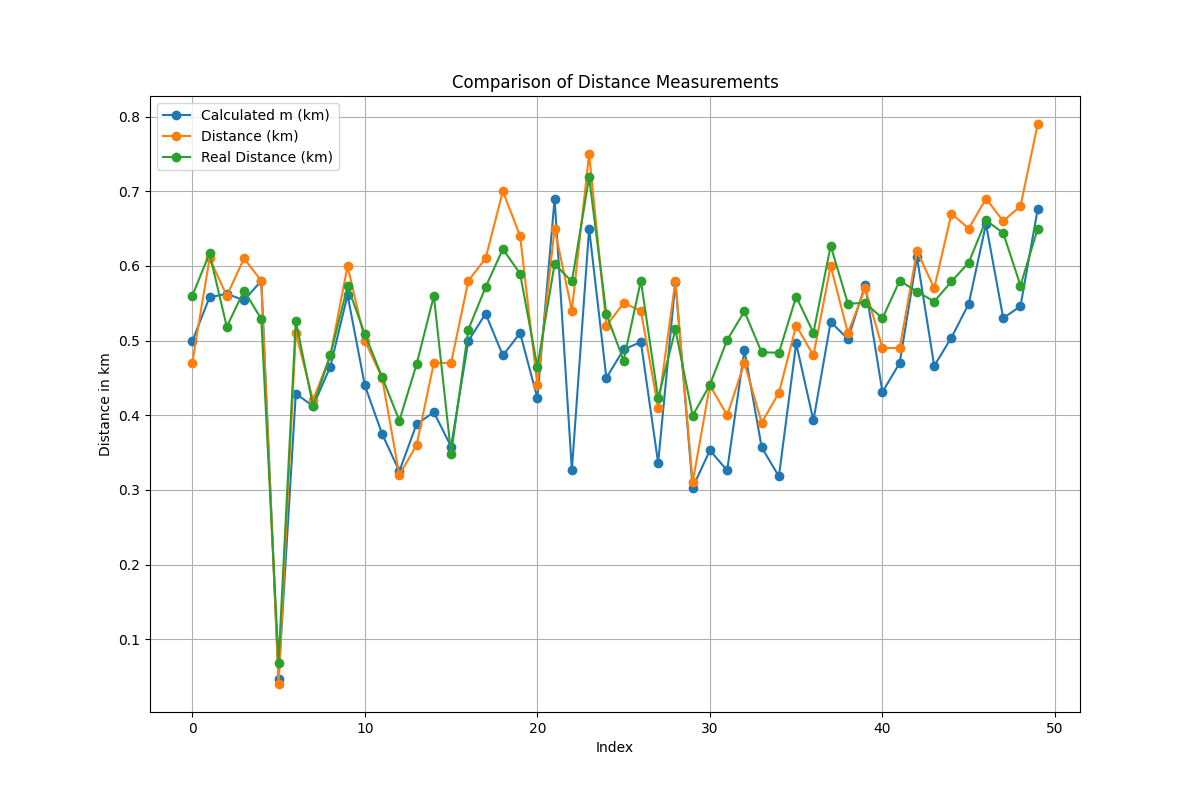
\includegraphics[width=0.9\textwidth]{Master Thesis/Plots/distance_comparison_plot.png}
    \caption{Comparison of measured distances 'Distance (km)', ’real_Distance’ and ’Calculated m’}
    \label{fig:distance_comparison_plot}
\end{figure}
\FloatBarrier

The differences between these measurements are calculated as percentages:
\begin{itemize}
    \item The highest difference between 'Calculated m' and 'Distance (km)' was 17.5\%.
    \item The highest difference between 'Calculated m' and 'real\_Distance' was 14.51\%.
    \item The highest difference between 'Distance (km)' and 'real\_Distance' was 34.94\%.
\end{itemize}

We have identified significant discrepancies between the actual distance traveled and the distance measured by the Apple Watch Ultra. Due to these large variations, we decided to use only the calculated distance for further analysis. This calculated distance is derived from the number of steps recorded by the Apple Watch Ultra and the leg length, thus partially utilizing Apple Watch Ultra data. Additionally, in this chapter, our focus is on using data measured by the Apple Watch Ultra to demonstrate that we can achieve better results.

\subsection{Additional Heart Rate and Blood Pressure Data}

To incorporate additional health metrics into our analysis, we decided to include blood pressure readings, as these provide valuable insights into a person's health. We manually added these values to the dataset from paper records and categorized them according to standard medical guidelines found online. These categories were then converted into numerical classes to facilitate their use in our models.

We categorized the blood pressure based on systolic (upper number) and diastolic (lower number) readings, measured in millimeters of mercury (mm Hg) ~\cite{heartUnderstandingBlood}:
\begin{itemize}
    \item \textbf{Normal blood pressure}: Systolic $<$ 120 mm Hg and diastolic $<$ 80 mm Hg, indicating a healthy heart condition and lower risk of cardiovascular diseases.
    \item \textbf{Elevated blood pressure}: Systolic 120-129 mm Hg and diastolic $<$ 80 mm Hg, indicating a higher than normal range but not yet hypertensive.
    \item \textbf{Hypertension Stage 1}: Systolic 130-139 mm Hg or diastolic 80-89 mm Hg, requiring lifestyle modifications and possibly medication.
    \item \textbf{Hypertension Stage 2}: Systolic $\geq$ 140 mm Hg or diastolic $\geq$ 90 mm Hg, necessitating more intensive treatment.
    \item \textbf{Hypertensive crisis}: Systolic $>$ 180 mm Hg and/or diastolic $>$ 120 mm Hg, a critical condition needing immediate medical intervention to prevent life-threatening complications such as organ damage or stroke.
\end{itemize}

We then added an additional column, alongside the columns for blood pressure before and after the 6MWT, to classify each subject's blood pressure. This classification helped us better understand the distribution of blood pressure among our subjects. The distribution of these categorized blood pressure values is illustrated in the following plot:

\FloatBarrier
\begin{figure}[h!]
    \centering
    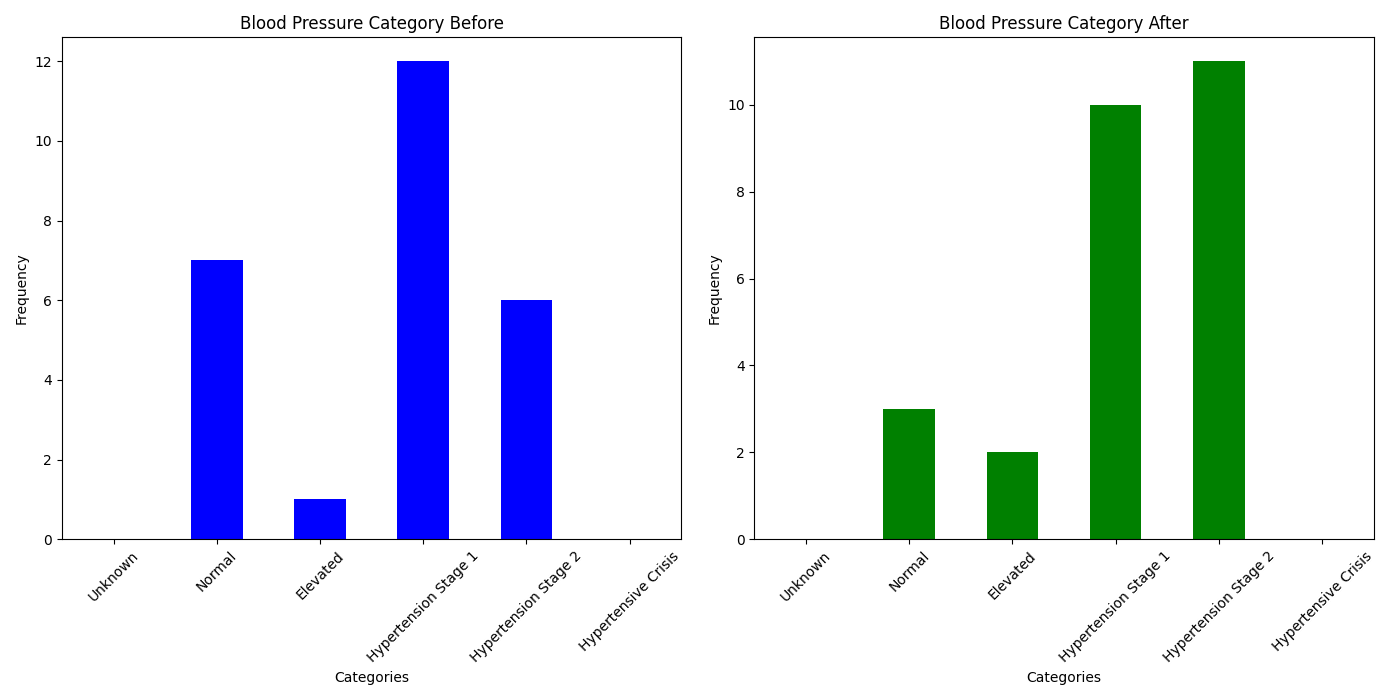
\includegraphics[width=1.0\textwidth]{Master Thesis/Plots/BloodPressure.png}
    \caption{Distribution of blood pressure categories}
    \label{fig:blood_pressure_distribution}
\end{figure}
\FloatBarrier

From the distribution, it is evident that there are no subjects in the 'Hypertensive Crisis' category, which is positive. However, a notable number of subjects fall into 'Hypertension Stage 1' and 'Hypertension Stage 2' categories, indicating a prevalence of elevated blood pressure and potential health risks within the study population. 

\subsection{Sex-Specific Data Analysis}

Additional information regarding the sex of the subjects was incorporated into the dataset from the documentation. We extracted details from the study, including sex and added them to the CSV file. One of our primary objectives was to investigate whether the heart rate of female subjects is generally higher than that of male subjects. To achieve an accurate analysis, we included 40 heart rate measurements for each subject in the dataset, with each value represented in a separate column. The information of the sex was manually entered as it was initially provided on paper.

The following plots visualize the measured heart rate for each male and female subject:

\FloatBarrier
\begin{figure}[h!]
  \centering
  \begin{minipage}[b]{0.9\linewidth}
    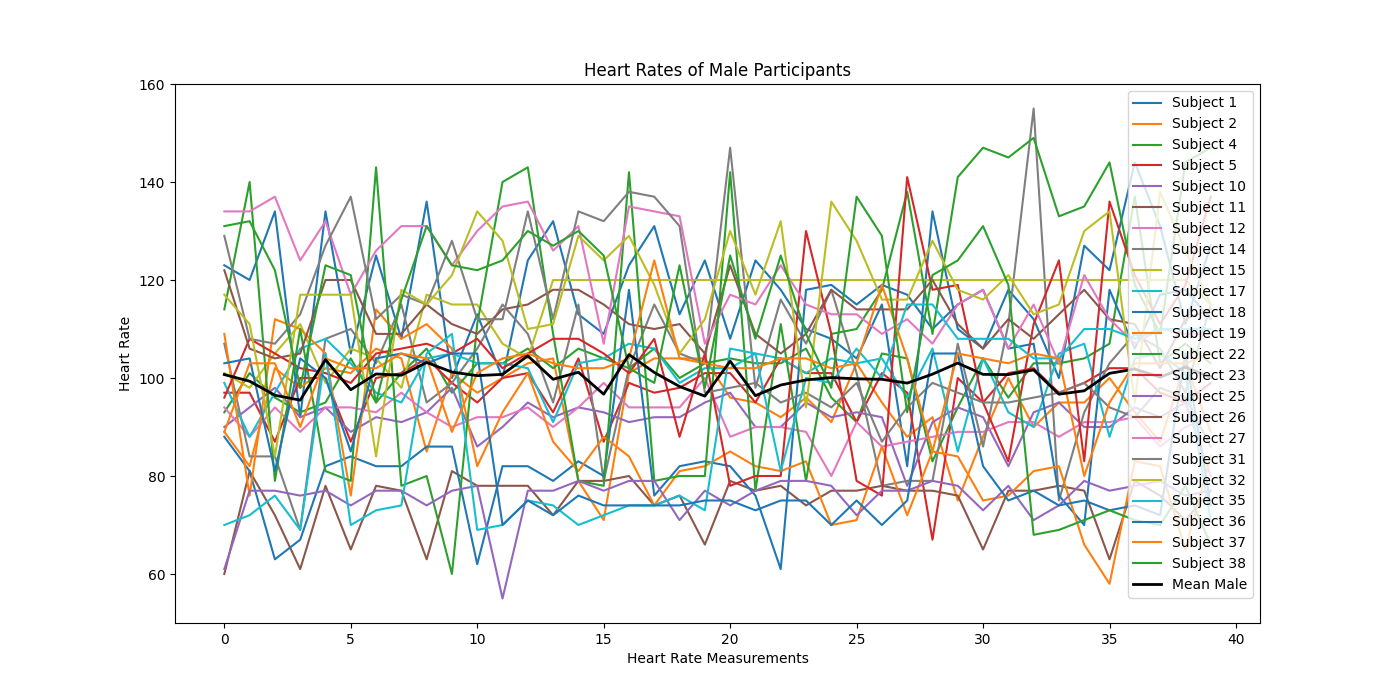
\includegraphics[width=\linewidth]{Master Thesis/Plots/comparison_plot_male.png}
    \caption{Visualization of the measured heart rate of each male subject and the measured mean in black}
    \label{fig:allmeashrdatamale}
  \end{minipage}
  \quad % Space between the images
  \begin{minipage}[b]{0.9\linewidth}
    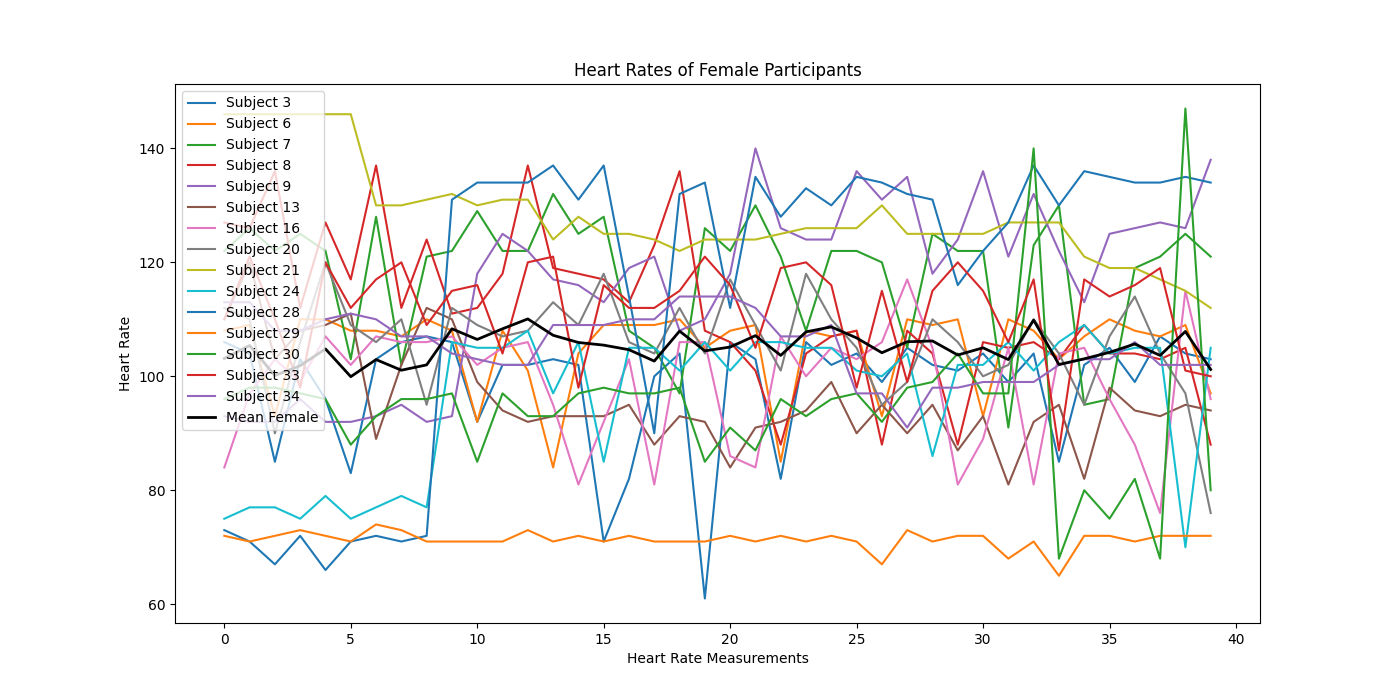
\includegraphics[width=\linewidth]{Master Thesis/Plots/comparison_plot_female.png}
    \caption{Visualization of the measured heart rate of each female subject and the measured mean in black}
    \label{fig:allmeashrdatafemale}
  \end{minipage}
\end{figure}
\FloatBarrier

Figure ~\ref{fig:allmeashrdatamale} and ~\ref{fig:allmeashrdatafemale} indicate that the heart rate patterns for both male and female subjects vary significantly. In each plot, individual lines represent the heart rate measurements for each subject across 40 instances. The black line represents the mean heart rate for all male and female subjects, providing a clear comparison of average heart rates between sex.

Figure ~\ref{fig:allmeashrdatafemale} presents the heart rates of female participants.
Each colored line represents the heart rate measurements of an individual female subject.
Similar to the male subjects in figure ~\ref{fig:allmeashrdatamale}, the black line represents the mean heart rate across all female subjects, indicating the overall trend and average heart rate pattern for females.

\FloatBarrier
\begin{figure}[h!]
  \centering
    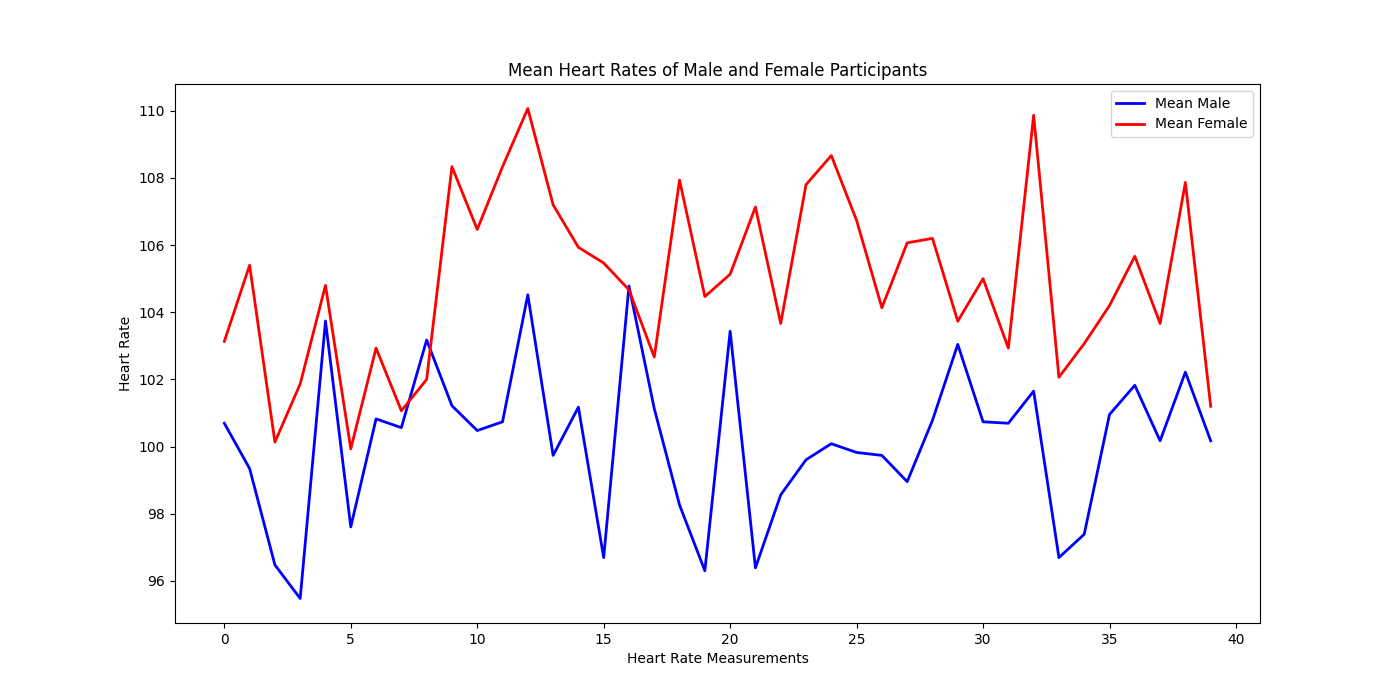
\includegraphics[width=1.0\linewidth]{Master Thesis/Plots/comparison_plot_mean_maleVSfemale.png}
    \caption{Mean heart rate comparison between male and female subjects}
    \label{fig:avhHRmalefemale}
\end{figure}
\FloatBarrier

Figure ~\ref{fig:avhHRmalefemale} highlights potential differences in cardiovascular responses between sex. It is evident that female subjects generally have higher mean heart rates compared to male subjects throughout the measurement period. This trend could indicate variations in cardiovascular health or fitness levels between the two groups. The fluctuations in the lines suggest variability in heart rates, with some overlap in certain intervals but a clear distinction in others. This visualization helps in understanding the general heart rate patterns and differences between male and female subjects.

\section{Supervised Learning Models}

We now evaluate the performance of supervised learning models on our dataset, including the information from the documentation and 10 heart rate measurements per subject. Our goal is to determine how well these models can predict health metrics based on this enriched data.

\subsection{Random Forest}
First we aimed to predict the sex of subjects using a combination of features including age, height, weight (not measured by the Apple Watch Ultra), and heart rates. We focused on the heart rates during the 6MWT, before, and after the test and even the blood pressure before and after the test. Utilizing the RF classifier model, we achieved an accuracy of 1.0. The detailed results are as follows:

\begin{table}[H]
\centering
\begin{tabular}{lrrrr}
\toprule
{} &  precision &  recall &  f1-score &  support \\
\midrule
female       &        1.0 &     1.0 &       1.0 &      2.0 \\
male         &        1.0 &     1.0 &       1.0 &      4.0 \\
macro avg    &        1.0 &     1.0 &       1.0 &      6.0 \\
weighted avg &        1.0 &     1.0 &       1.0 &      6.0 \\
\bottomrule
\end{tabular}
\caption{RF sex classification with all given features and 10 heart rate values}
\label{table:RFageHeartrate10weightheigt}
\end{table}

The results in table ~\ref{table:RFageHeartrate10weightheigt} from the RF model for predicting sex achieves perfect scores across all metrics. The precision of the model is 1.0 for both female and male subjects, indicating that every prediction made by the model for both sex was correct. The recall is also 1.0 for both female and male subjects, meaning that the model successfully identified all actual instances of both sex. The f1-score, which is the harmonic mean of precision and recall, is 1.0 for both sex, reflecting the model's perfect balance between precision and recall.

The support indicates the number of actual instances for each class in the test set, with two instances of female and four instances of male subjects. The overall accuracy of the model is 1.0, meaning the model correctly predicted the sex for all subjects in the test set. Both macro average and weighted average for precision, recall, and f1-score are also perfect at 1.0, demonstrating that the model performs consistently well across both classes.

These outstanding results suggest that the chosen features (age, height, weight, and heart rates) are highly effective in predicting sex. To further understand these results, we analyzed the importance of each feature in the model's decision-making process. The following plot illustrates the feature importance in the sex predictions:

\FloatBarrier
\begin{figure}[h!]
    \centering
    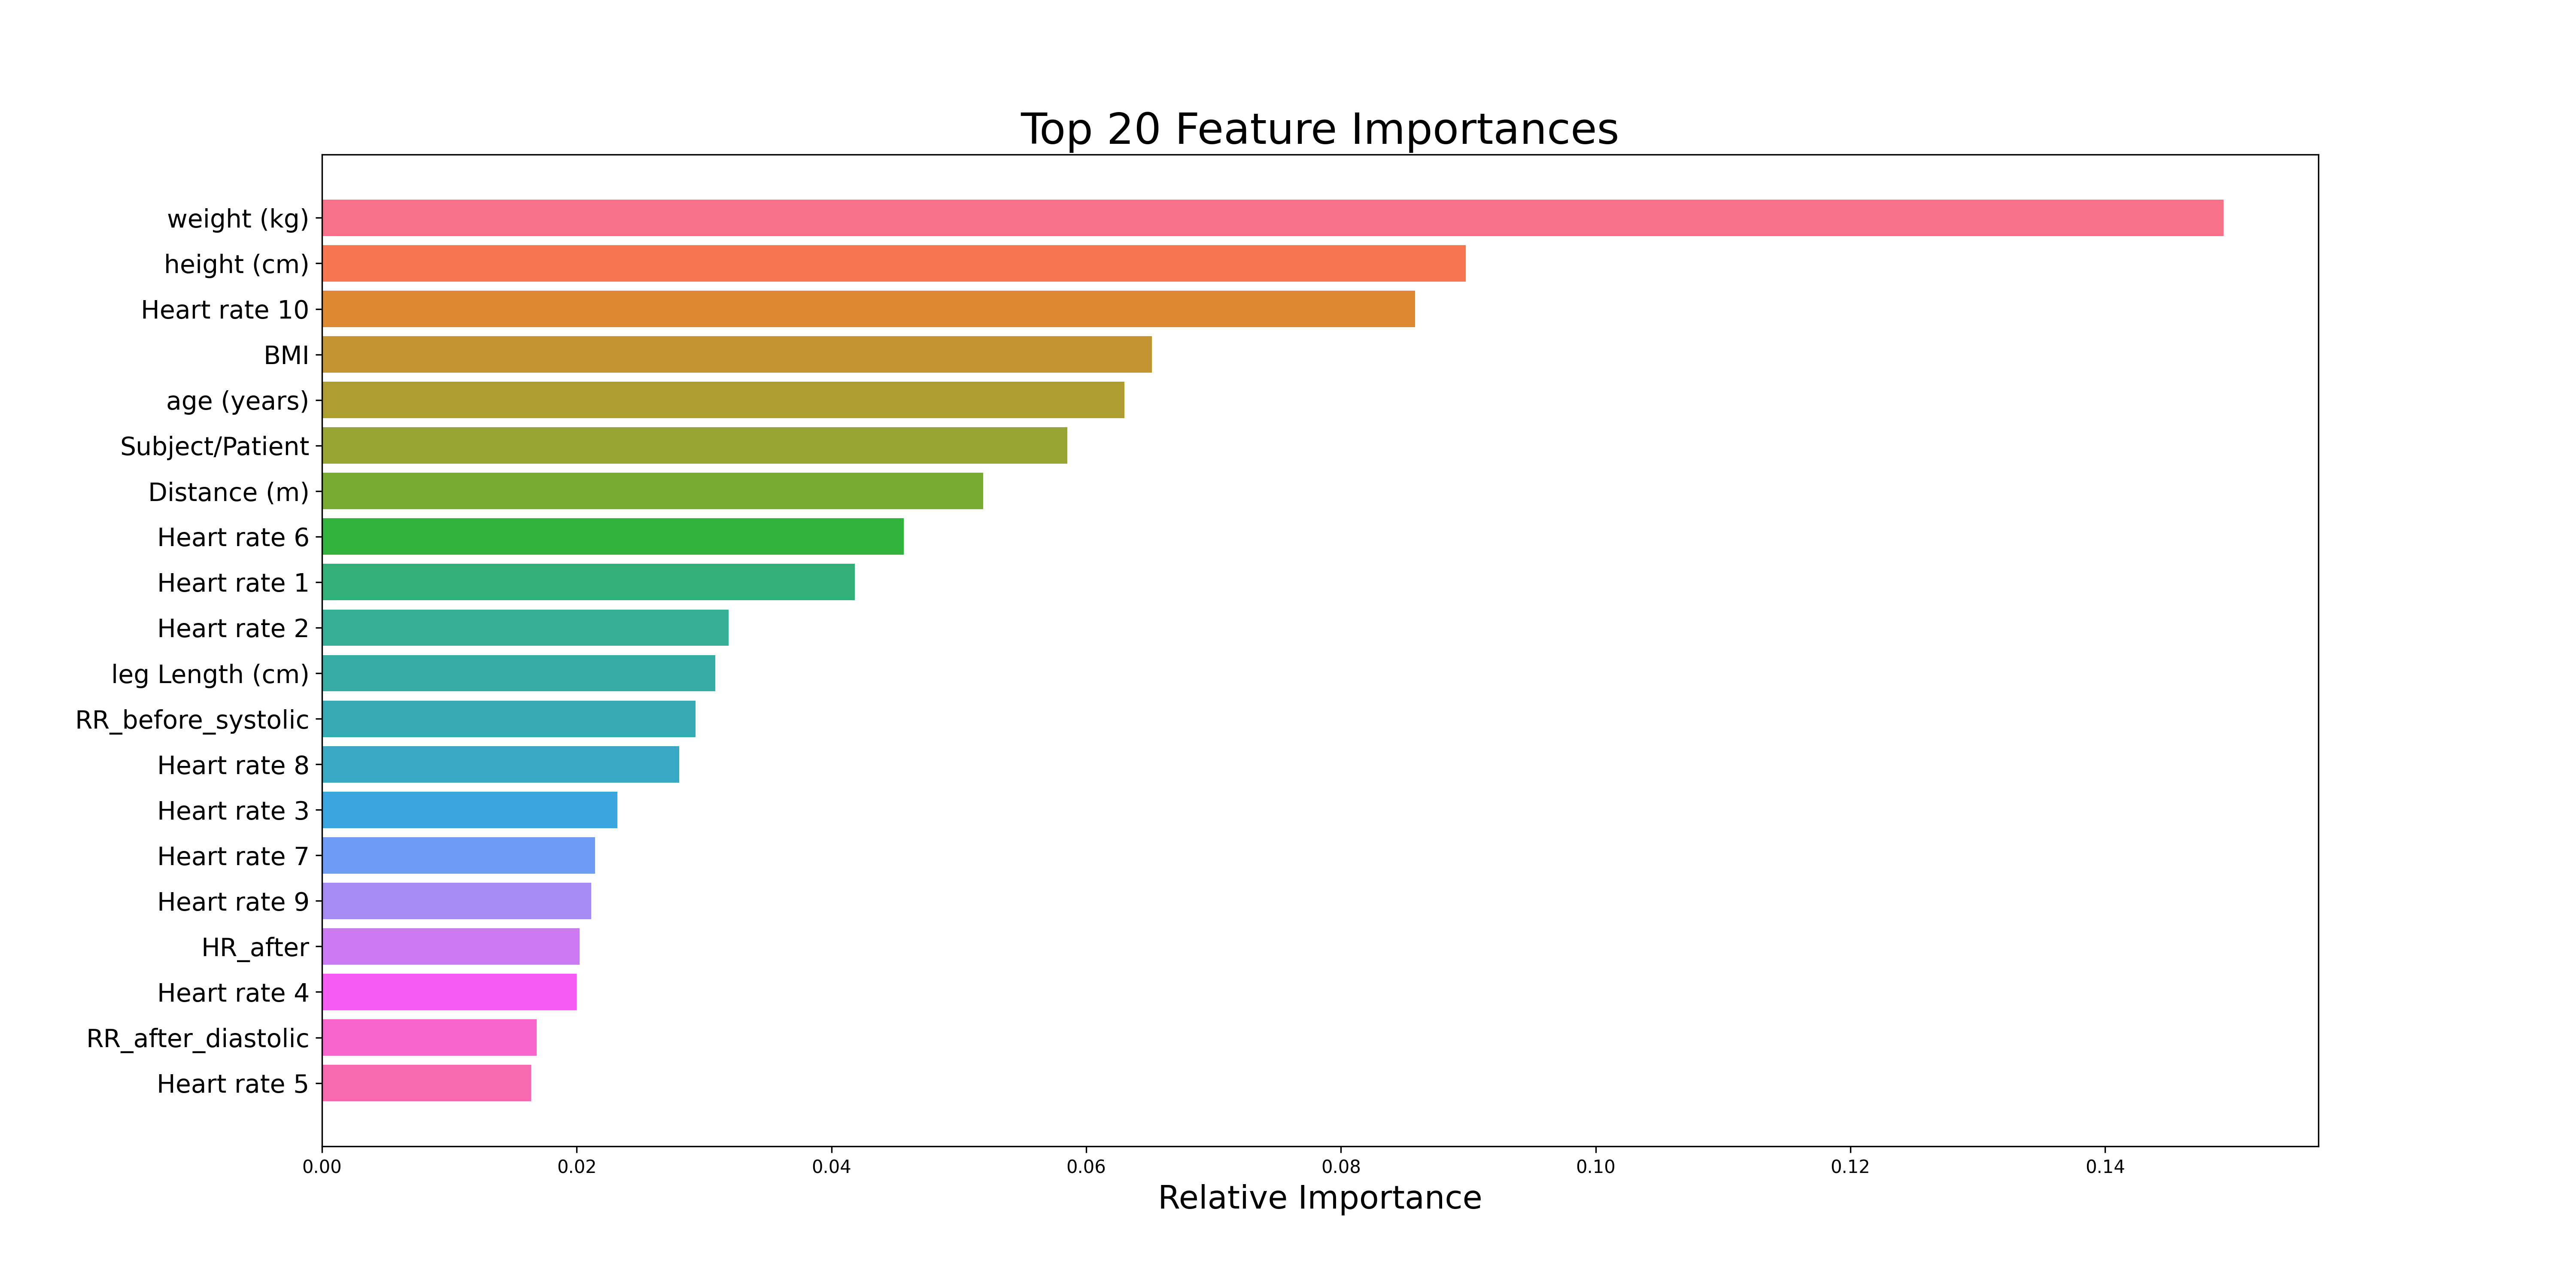
\includegraphics[width=1.0\textwidth]{Master Thesis/Plots/random_forest_top20_feature_importances_gender_oldData.png}
    \caption{Feature importance for sex prediction using RF with all given features and 10 heart rate values}
    \label{fig:featureimportanceRFsex10}
\end{figure}
\FloatBarrier

Figure ~\ref{fig:featureimportanceRFsex10} reveals that height and weight are the most important features for accurate sex prediction. Additionally, heart rates, particularly the latest measurements, age, and blood pressure before and after the 6MWT, are essential for achieving a perfect score with the RF model. As well we added features like active and basal energy burned. We have added these functions by summing up all the values of the energy type, whether basal or active. These are all values measured by the Apple Watch Ultra.

The supposedly excellent results are still questionable. Because of the six most important features for the prediction, only one feature is measured by the Apple Watch Ultra. However, we want to show that the Apple Watch Ultra delivers good and, above all, important data for the ML area, so we need to make further optimizations here. We expanded the dataset with additional heart rate data (100 measured heart rate values per subject) and another feature, to predict the sex of the subjects. This model achieved an accuracy of 78\%. The detailed results are shown below:

\begin{table}[H]
\centering
\begin{tabular}{lrrrr}
\toprule
{} &  precision &    recall &  f1-score &   support \\
\midrule
male            &   0.71 &  1.00 &  0.83 &  5.0 \\
female            &   1.00 &  0.50 &  0.67 &  4.0 \\
macro avg    &   0.86 &  0.75 &  0.75 &  9.0 \\
weighted avg &   0.84 &  0.78 &  0.76 &  9.0 \\
\bottomrule
\end{tabular}
\caption{RF sex classification with all given features and 100 heart rate values}
\label{table:RFageHeartrate100weightheigt}
\end{table}

The results from the RF classifier in table ~\ref{table:RFageHeartrate100weightheigt} with additional features are promising. The precision for class 'male' is 0.71, with a recall of 1.00, indicating that the model correctly identified all instances of this class. The f1-score for class 'male' is 0.83. For class 'female', the precision is 1.00, with a recall of 0.50, and an f1-score of 0.67.

Overall, the model achieved an accuracy of 0.78, meaning it correctly predicted the risk classification for 78\% of the subjects in the test set. The macro averages for precision, recall, and f1-score are 0.86, 0.75, and 0.75, respectively. The weighted averages are 0.84 for precision, 0.78 for recall, and 0.76 for f1-score.

These results suggest that the additional features have enhanced the model's predictive capability. To understand the impact of each feature, we analyzed their importance in the model's decision-making process. The following graph illustrates the feature importance:
\FloatBarrier
\begin{figure}[h!]
    \centering
    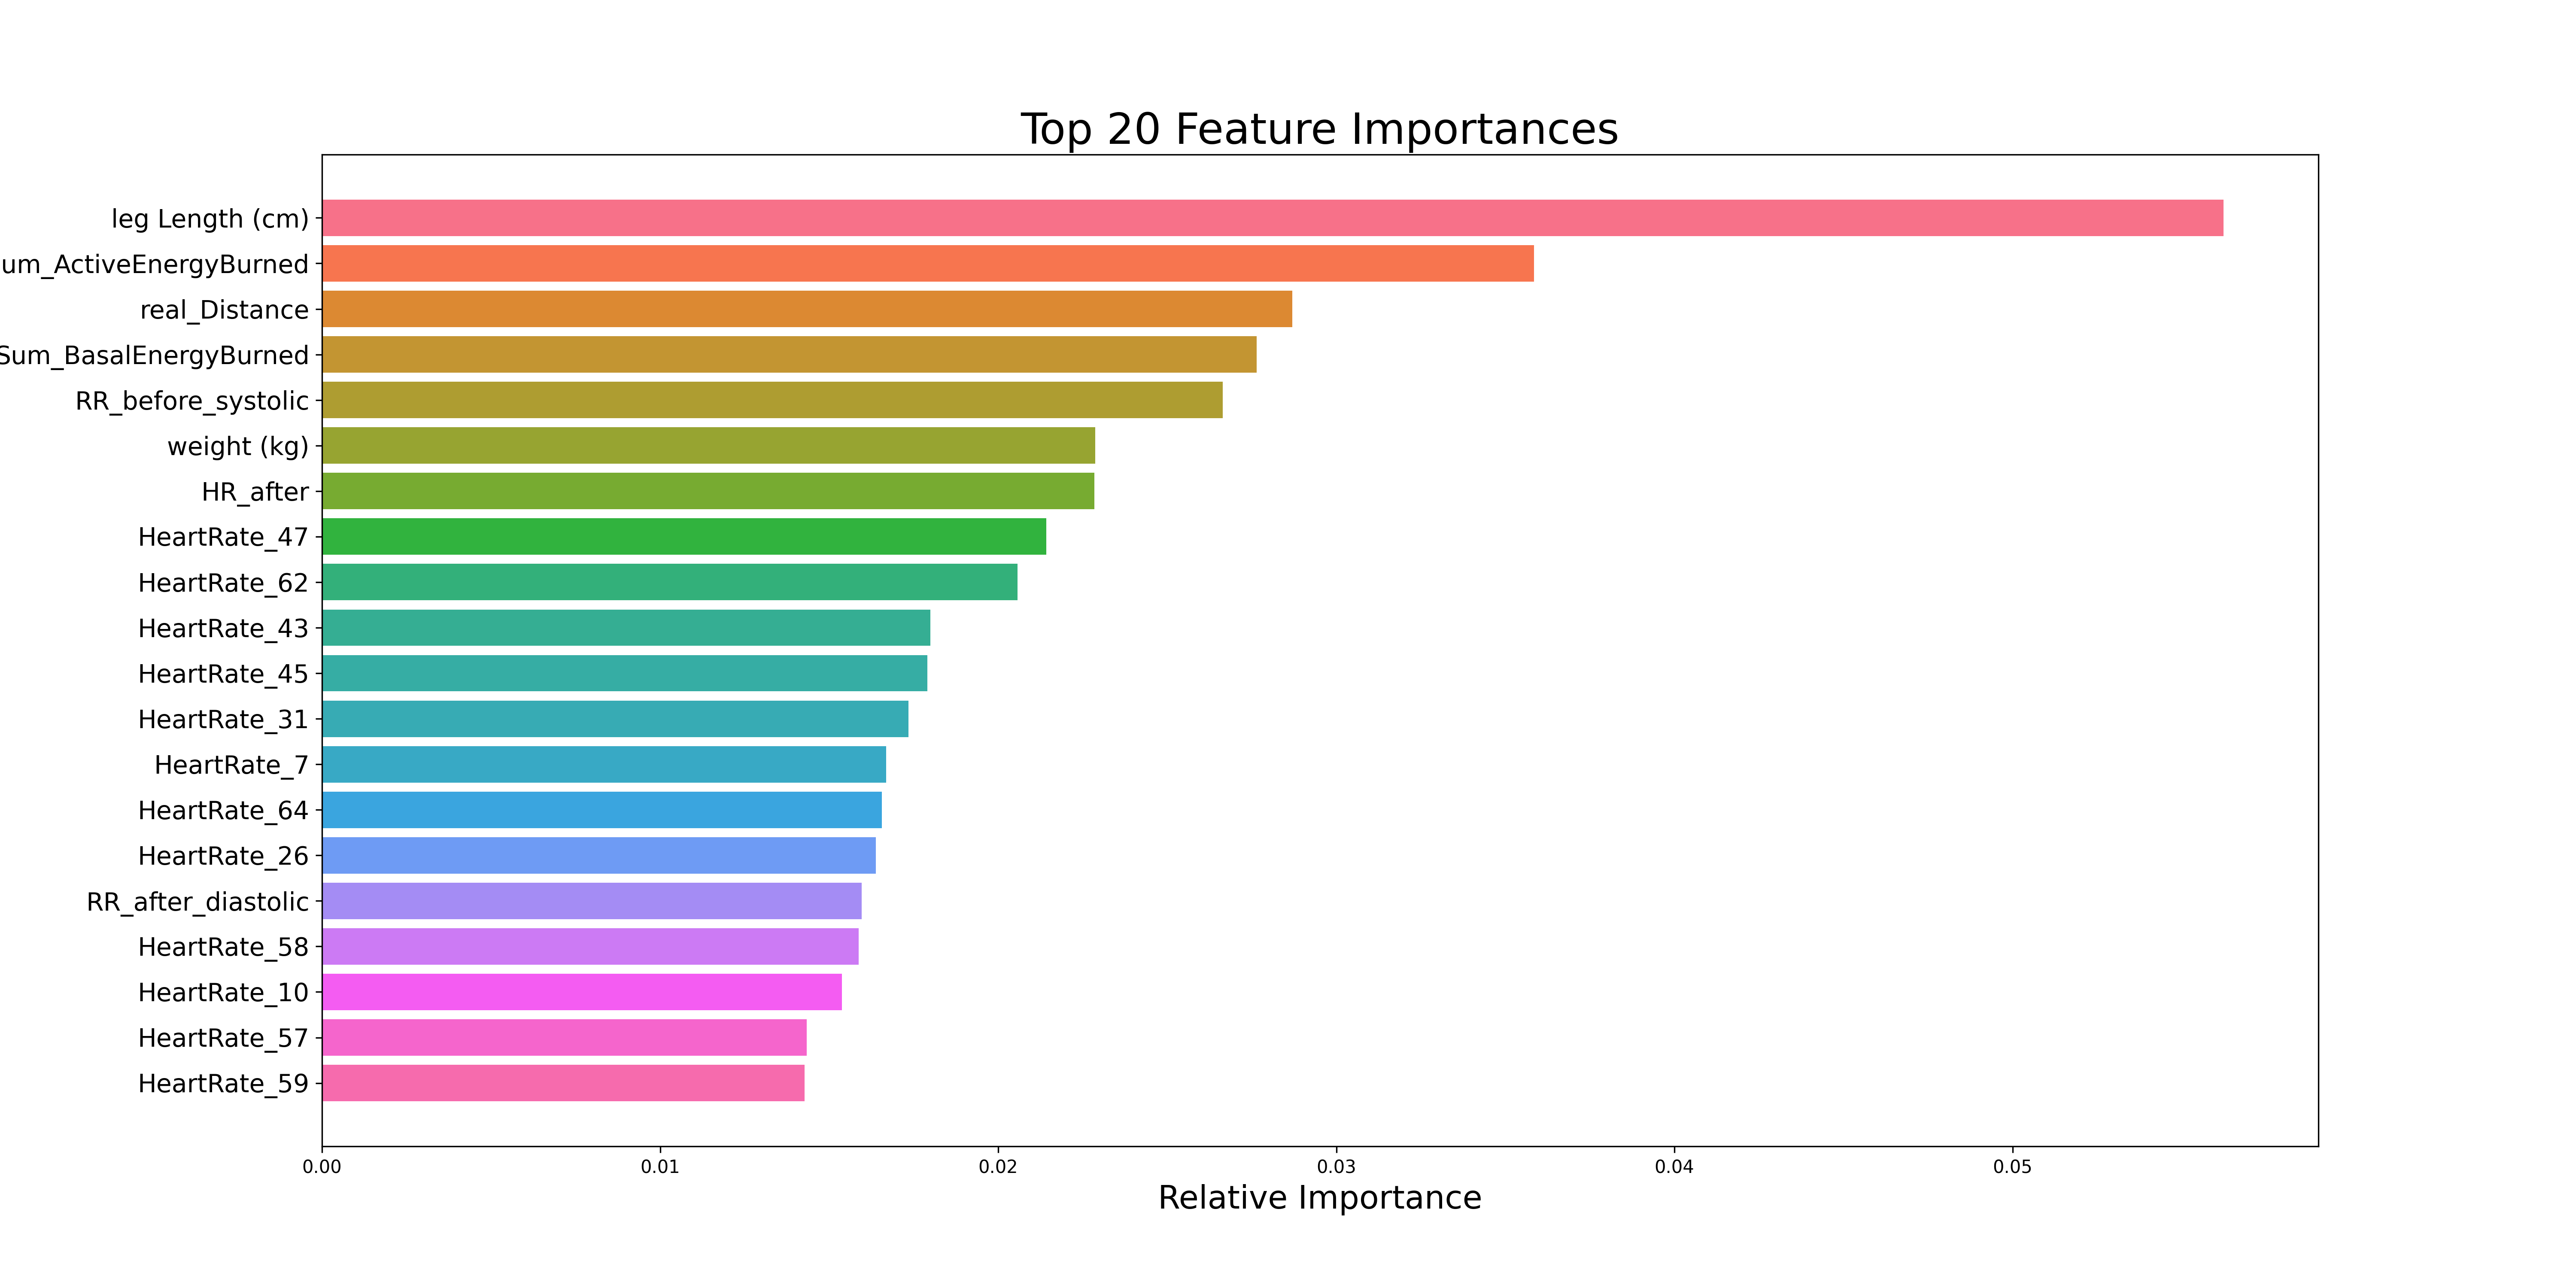
\includegraphics[width=1.0\textwidth]{Master Thesis/Plots/random_forest_top20_feature_importances_gender.png}
        \caption{Feature importance for sex prediction using RF with all given features and 100 heart rate values}
    \label{fig:featureimportanceRFsex100}
\end{figure}
\FloatBarrier

Figure ~\ref{fig:featureimportanceRFsex100} confirms the importance of height, weight, and various heart rate measurements, along with additional features like burned calories, in predicting sex. The results demonstrate the significant impact of these features on the accuracy of the RF model. And shows on the other hand that we did a prediction where the most important features where measured by the Apple Watch Ultra, what we wanted to show.

\subsubsection{Subject or Patient Classification with Random Forest}

We aimed to replicate the subject or patient prediction from chapter ~\ref{cha:results} and assess how the new features impact the results. We again started with the features the same as for table ~\ref{table:RFageHeartrate10weightheigt}, but instead of predicting sex, we predicted whether an individual is a subject or patient. Using a RF model, we achieved an accuracy of 0.83. The detailed results are as follows:

\begin{table}[H]
\centering
\begin{tabular}{lrrrr}
\toprule
{} &  precision &    recall &  f1-score &   support \\
\midrule
subject      &   0.75 &  1.00 &  0.86 &  3.0 \\
patient      &   1.00 &  0.67 &  0.80 &  3.0 \\
macro avg    &   0.88 &  0.83 &  0.83 &  6.0 \\
weighted avg &   0.88 &  0.83 &  0.83 &  6.0 \\
\bottomrule
\end{tabular}
\caption{RF subject or patient classification with all given features and 10 heart rate values}
\label{table:featureimportanceRFsubpat10}
\end{table}

The results from the RF model for predicting whether an individual is a subject or a patient are summarized in the table. The model achieved an accuracy of 0.83. The precision for predicting 'subject' is 0.75 with a recall of 1.00, resulting in an f1-score of 0.86. For predicting 'patient' the precision is 1.00 with a recall of 0.67, yielding an f1-score of 0.80. The macro average for precision, recall, and f1-score are 0.88, 0.83, and 0.83 respectively. The weighted average for all these metrics is also 0.88, 0.83, and 0.83 respectively. These results indicate a strong model performance with balanced precision and recall across both classes.

The feature importance plot provides insights into which features contributed most to the model's performance:

\FloatBarrier
\begin{figure}[h!]
    \centering
    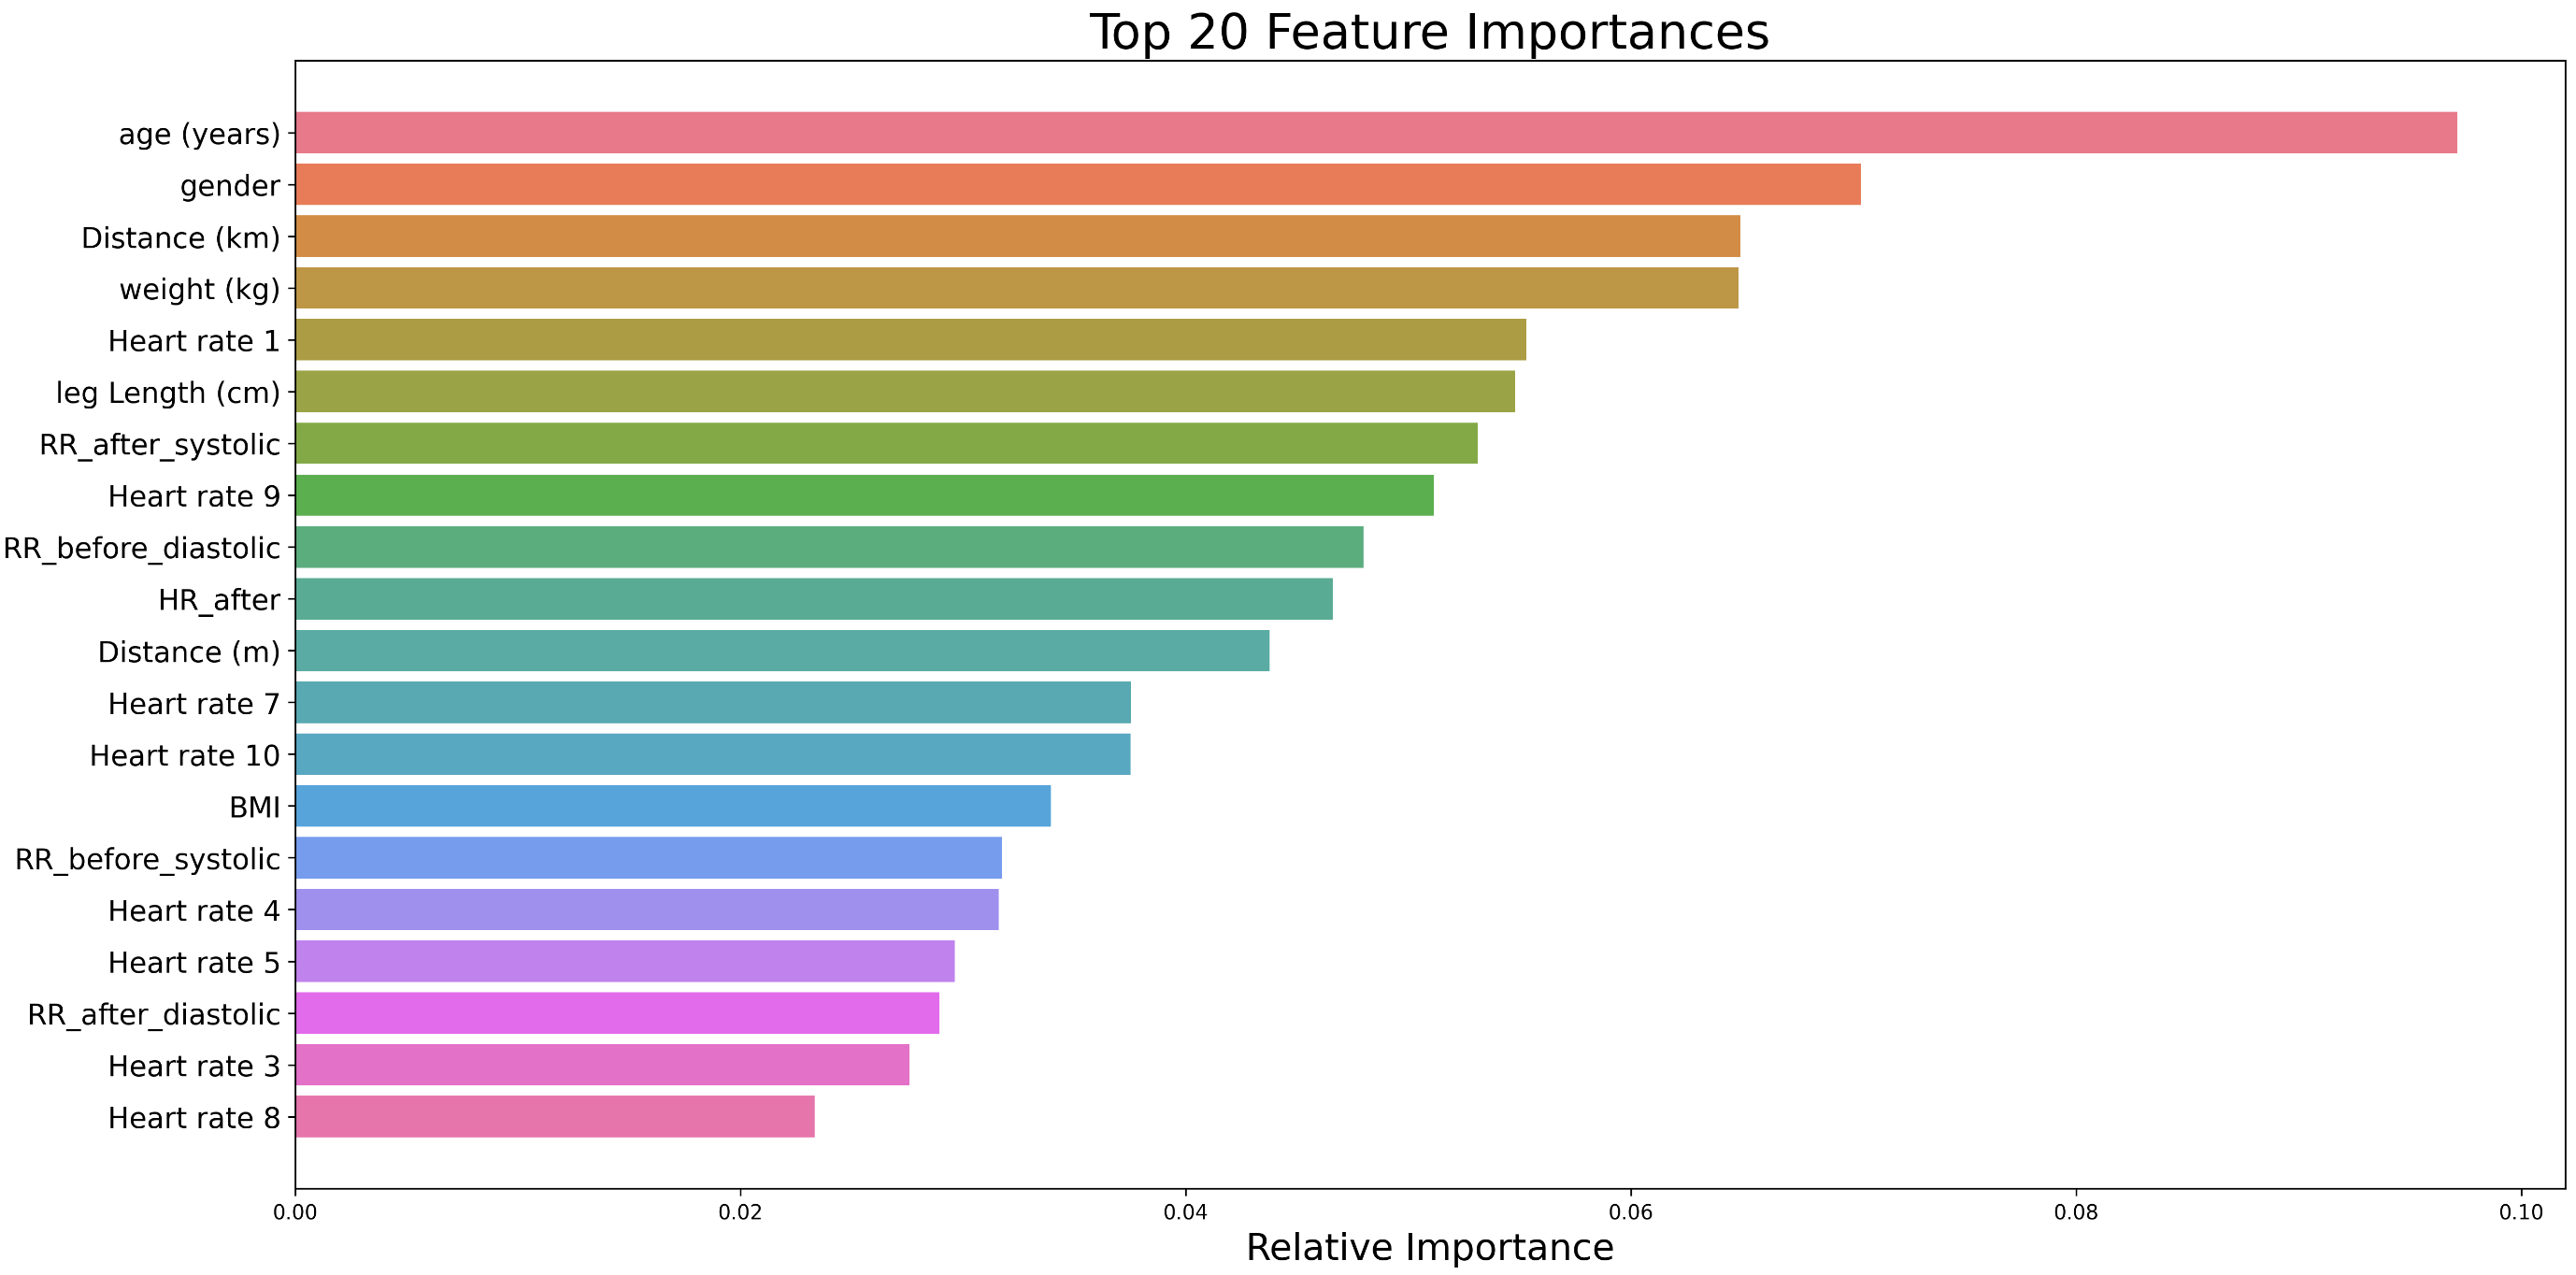
\includegraphics[width=1.0\textwidth]{Master Thesis/Plots/random_forest_top20_feature_importances_subjpatient.png}
    \caption{Feature importance for subject or patient prediction using RF with all given features and 10 heart rate values}
    \label{fig:featureimportanceRFsubpat10}
\end{figure}
\FloatBarrier

Figure ~\ref{fig:featureimportanceRFsubpat10} reveals that age, blood pressure before and after the 6MWT, and the first measured heart rate are key features for achieving a relatively accurate prediction. The importance of these features emphasizes that the Apple Watch Ultra provides relevant and important measurements that are essential for predictions.

After expanding the dataset to include the 100 heart rate measurements for each subject, sorted sequentially and added to the table, the model achieved an accuracy of 100\%, as detailed below:

\begin{table}[H]
\centering
\begin{tabular}{lrrrr}
\toprule
{} &  precision &  recall &  f1-score &  support \\
\midrule
subject            &        1.0 &     1.0 &       1.0 &      6.0 \\
patient            &        1.0 &     1.0 &       1.0 &      3.0 \\
macro avg    &        1.0 &     1.0 &       1.0 &      9.0 \\
weighted avg &        1.0 &     1.0 &       1.0 &      9.0 \\
\bottomrule
\end{tabular}
\caption{RF subject or patient classification with all given features and 100 heart rate values}
\label{table:featureimportanceRFsubpat100}
\end{table}

The classification results with the expanded dataset demonstrate exceptional performance, achieving a perfect accuracy of 100\%. Both precision and recall for each class are 1.0, indicating that the model correctly identified all instances without any errors. The macro and weighted averages also reflect perfect scores, underscoring the model's robustness and reliability in predicting the subject or patient status.

The feature importance for this model is shown in the following plot:

\FloatBarrier
\begin{figure}[h!]
    \centering
    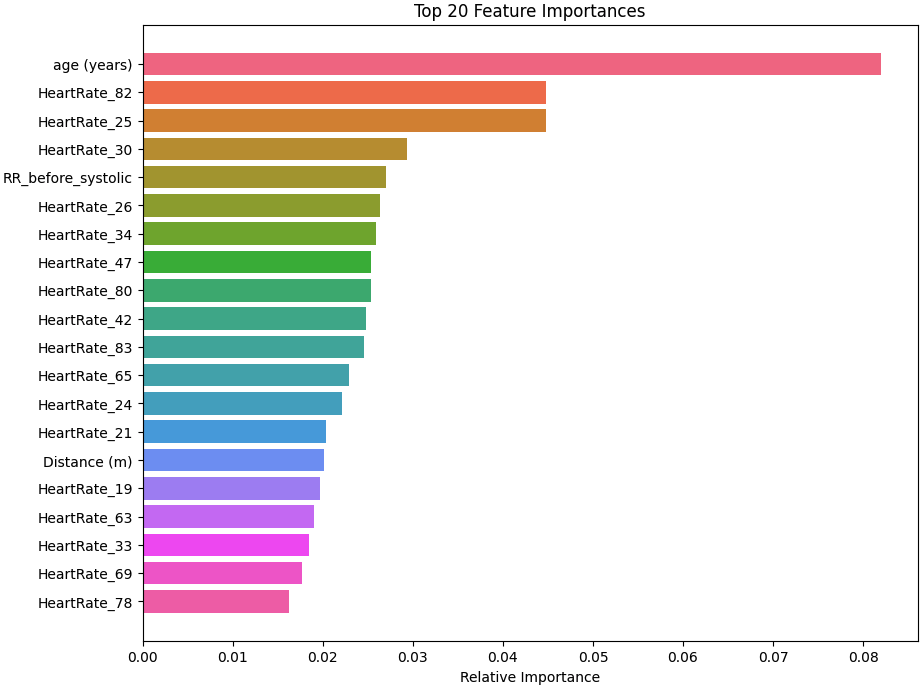
\includegraphics[width=1.0\textwidth]{Master Thesis/Plots/Random_forest_top20_patientsubject.png}
    \caption{Feature importance for subject or patient prediction using RF with all given features and 100 heart rate values}
    \label{table:featureimportanceRFsubpat100}
\end{figure}
\FloatBarrier

The feature importance figure ~\ref{table:featureimportanceRFsubpat100} shows that age is the most important factor, followed by several heart rate measurements. This emphasizes the importance of combining various features for the best prediction accuracy.

Achieving an accuracy of 100\% often means our model might be overfitting. To check this, we trained a model using only the 'age' feature, and the accuracy dropped to 88\%. This shows that age is important, but we also need other features for better predictions.

In summary, our results show that we need a full set of features for accurate predictions. While age is a strong predictor, adding other health metrics like blood pressure and heart rate improves the model. The feature importance plot below highlights the value of using different physiological and demographic factors for better accuracy. Future models will be better with larger datasets and more refined feature selection.

\subsection{Regression}

Since linear regression did not perform well with the data from chapter ~\ref{cha:results}, we decided to skip it in this chapter and directly look for optimizations or at least alternatives, hoping for better results. We started with the XGBoost model. To get a better understanding of how it compares to linear regression before applying it to our entire dataset, we first tested it on a small dataset with only a few data points.

Beside the distribution of the categories, a deeper analysis was conducted on various regression models and their outcomes. The results of the linear regression were particularly disappointing, yielding a poor RMSE value of 0.63. In contrast, the XGBoost model demonstrated significantly better performance with an RMSE value of 0.16. The generated plots are presented below:

\FloatBarrier
\begin{figure}[h]
    \centering
    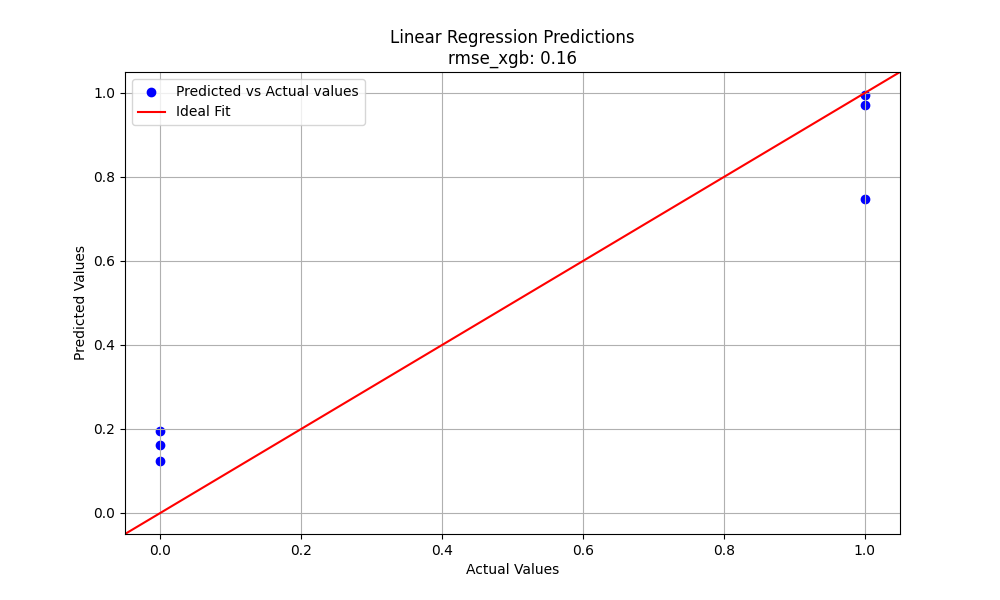
\includegraphics[width=0.75\textwidth]{Master Thesis/Plots/XG_boost_bloodPressure.png}
    \hspace{0.5cm} % Abstand zwischen den Bildern
    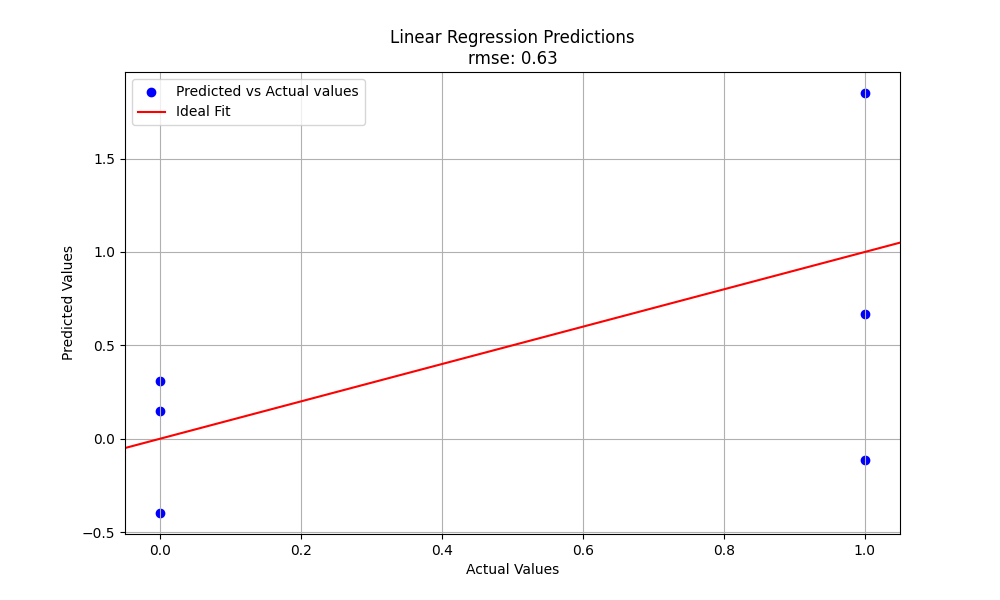
\includegraphics[width=0.75\textwidth]{Master Thesis/Plots/linReg_bloodPressure.png}
    \caption{Comparison of linear regression and XGBoost with a random part of the dataset}
    \label{fig:complinregXGBoost}
\end{figure}
\FloatBarrier

Figure ~\ref{fig:complinregXGBoost} reveals a significant difference in the performance of the two models. The XGBoost model, indicated by the plot on the top, shows blue dots clustered closely along the ideal fit line, highlighting the accuracy of the predictions. The RMSE value of 0.16 underscores the model's precision in predicting whether an individual is a subject or a patient.

On the other hand, the linear regression model, depicted in the bottom plot, shows a less favorable distribution of blue dots, which are spread farther from the ideal fit line. This is reflected in the higher RMSE value of 0.63, indicating poor predictive performance. Given that the prediction involves binary outcomes (zero and one), an RMSE of 0.63 suggests a high level of inaccuracy, making the linear regression model unreliable for this task.

In summary, the XGBoost model significantly outperforms the linear regression model, providing more accurate and reliable predictions for classifying individuals as subjects or patients based on the given features. Therefore, we will not proceed with XGBoost on our current dataset but will focus on exploring additional models to improve our predictions.

\subsubsection{Ridge Regression}
Ridge regression is particularly suitable for datasets with multicollinearity or when there are a large number of features, such as heart rate measurements in our dataset. We hoped for even better results using this regression. In the context of our study, where the dataset now consists primarily of various heart rate readings, it is essential to consider a regression model that can handle the potential collinearity among these features and provide robust predictions. Ridge regression achieves this by adding a regularization term to the loss function, which helps in managing the weights of the features effectively, preventing overfitting, and ensuring that the model remains transferable to new data. This is especially important when dealing with heart rate data, which can have many correlated variables.

Subsequently, a weighted regression analysis was performed using all measured heart rates to predict age. The results are detailed below:

\begin{table}[H]
\begin{longtable}{|>{\raggedright}p{4cm}|>{\raggedright\arraybackslash}p{10cm}|}
\hline
\textbf{metric} & \textbf{value} \\
\hline
\endfirsthead
\hline
\textbf{metric} & \textbf{value} \\
\hline
\endhead
\hline
\endfoot
ridge regression coefficients & 
\begin{minipage}[t]{10cm}
[  9.65, \   2.27, \  -5.39, \  -3.84, \   1.63, \  -2.23, \   0.25, \   6.57, \   5.23, \ -12.42, \   3.52, \  -4.34, \   8.86, \   5.17, \   0.05]
\end{minipage}
\\
\hline
ridge regression intercept & 45.33 \\
\hline
R\textsuperscript{2} on test set & 0.62 \\
\hline
MSE & 209.79 \\
\hline
RMSE & 14.48 \\
\hline
CV scores & 
\begin{minipage}[t]{10cm}
[-0.07, \ -0.56, \ -1.51, \  0.46, \ -0.34]
\end{minipage}
\\
\hline
mean CV score & -0.41 \\
\hline
\end{longtable}
\caption{Age prediction results with ridge regression based on all measured heart rates}
\label{tab:RRAgeallheart}
\end{table}

The ridge regression model for predicting age yielded a moderately good performance with an \( R^2 \) value of 0.62, explaining 62\% of the variability in the test dataset. The coefficients ranged from -12.42 to 9.65, indicating varying impacts of heart rate measurements on age prediction, with an intercept starting at 45.33. The MSE was 209.79, and the RMSE was 14.48, indicating an average prediction error of about 14.48 years. However, the CV scores ranged from -0.07 to -1.51, with a mean score of -0.41, highlighting inconsistency and potential overfitting or underfitting issues. Overall, while the model showed moderate success, its inconsistency across different subsets of data suggests the need for further refinement or alternative models.

We are satisfied with the results so far and now want to investigate the results of predicting other characteristics. The prediction of the weight with the 100 heart rate values using ridge regression provided promising results:

\begin{table}[H]
\begin{longtable}{|>{\raggedright}p{4cm}|>{\raggedright\arraybackslash}p{10cm}|}
\hline
\textbf{metric} & \textbf{value} \\
\hline
\endfirsthead
\hline
\textbf{metric} & \textbf{value} \\
\hline
\endhead
\hline
\endfoot
ridge regression coefficients & 
\begin{minipage}[t]{10cm}
[ 1.57, \  1.15, \ -0.24, \ -0.77, \  0.03, \  2.14, \  0.04, \  6.56, \  0.16, \ -0.66, \  0.49, \  4.97, \ -0.73, \  3.56, \  0.33]
\end{minipage}
\\
\hline
ridge regression intercept & 76.86 \\
\hline
ridge regression R\textsuperscript{2} on test set & 0.94 \\
\hline
MSE & 12.74 \\
\hline
RMSE & 3.57 \\
\hline
CV scores & 
\begin{minipage}[t]{10cm}
[0.59, \ 0.90, \ 0.67, \ 0.98, \ 0.87]
\end{minipage}
\\
\hline
mean CV score & 0.80 \\
\hline
\end{longtable}
\caption{Weight prediction results with ridge regression based on all measured heart rates}
\label{tab:RRweightallheart}
\end{table}

The weight prediction model performs exceptionally well, with an \( R^2 \) value of 0.94, indicating that the model explains 94\% of the variability in the test dataset. The high mean CV score of 0.80 further supports the model's robustness and reliability. The ridge regression coefficients show the importance of various features, with the intercept at 76.86. The model achieved a MSE of 12.74 and a RMSE of 3.57, demonstrating its accuracy in predicting weight.

The results of predicting BMI using ridge regression, utilizing all heart rate measurements recorded by the Apple Watch Ultra and additional non-Apple Watch Ultra data such as leg length, are detailed below:

\begin{table}[H]
\begin{longtable}{|>{\raggedright}p{4cm}|>{\raggedright\arraybackslash}p{10cm}|}
\hline
\textbf{metric} & \textbf{value} \\
\hline
\endfirsthead
\hline
\textbf{metric} & \textbf{value} \\
\hline
\endhead
\hline
\endfoot
ridge regression coefficients & 
\begin{minipage}[t]{10cm}
[ 0.56, \  0.20, \  -0.57, \ -0.07, \ -0.27, \  1.51, \  1.68, \ -0.13, \ -0.31, \  0.98, \  0.23, \ -0.37, \ -1.53, \  0.94, \ -0.31]
\end{minipage}
\\
\hline
ridge regression intercept & 25.04 \\
\hline
ridge regression R\textsuperscript{2} on test set & 0.21\\
\hline
MSE & 8.48 \\
\hline
RMSE & 2.91 \\
\hline
CV scores & 
\begin{minipage}[t]{10cm}
[0.62, \ 0.79, \ 0.84, \ 0.91, \ 0.00]
\end{minipage}
\\
\hline
mean CV score & 0.63 \\
\hline
\end{longtable}
\caption{BMI prediction results with ridge regression based on all measured heart rates}
\label{tab:RRBMIallheart}
\end{table}

The BMI prediction model demonstrates moderate performance. The ridge regression coefficients shows varying impacts of features on predicted BMI values. The ridge regression intercept is 25.04, and the \( R^2 \) value on the test set is 0.21, indicating the model explained only 21\% of the variability in the test data. The MSE is 8.48, and the RMSE is 2.91, reflecting prediction errors. CV scores ranged from 0.00 to 0.91, with a mean score of 0.63, suggesting reasonable but improvable performance. Overall, the model shows some predictive capability, but further optimization is needed.

Lastly, we attempted to predict height with all the given information, but the results were not as promising:

\begin{table}[H]
\begin{longtable}{|>{\raggedright}p{4cm}|>{\raggedright\arraybackslash}p{10cm}|}
\hline
\textbf{metric} & \textbf{value} \\
\hline
\endfirsthead
\hline
\textbf{metric} & \textbf{value} \\
\hline
\endhead
\hline
\endfoot
ridge regression coefficients & 
\begin{minipage}[t]{10cm}
[-1.09, \  0.04, \  1.75, \ -0.46, \  0.37, \  0.39, \  6.46, \  1.59, \  0.51, \ -3.72, \ -0.78, \ -1.9, \  5.77, \ -0.24, \  0.83]
\end{minipage}
\\
\hline
ridge regression intercept & 173.83 \\
\hline
ridge regression R\textsuperscript{2} on test set & -0.66\\
\hline
MSE & 105.23 \\
\hline
RMSE & 10.26 \\
\hline
CV scores & 
\begin{minipage}[t]{10cm}
[-0.13, \  0.74, \ -5.28, \  0.63, \ -0.22]
\end{minipage}
\\
\hline
mean CV score & -0.85 \\
\hline
\end{longtable}
\caption{Height prediction results with ridge regression based on all measured heart rates}
\label{tab:RRHeightallheart}
\end{table}

The height prediction model performed poorly, with an \( R^2 \) value of -0.66, indicating that the model explains very little of the variability in the test dataset. The MSE is 105.23, resulting in a RMSE of 10.26. The CV scores also varied significantly, with a mean score of -0.85, further highlighting the model's inadequacy in predicting height based on the given data.

\subsection{Weighted Linear Regression}

We decided to give linear regression another try, but given the complexity and volume of heart rate data, the standard linear regression approach wouldn't work effectively. This led us to explore weighted linear regression, a model that adjusts the influence of different data points by assigning weights, making it more suitable for datasets with varying importance among features.

We used heart rate data, along with features such as BMI, weight, and height for feature selection. We applied Principal Component Analysis (PCA) to reduce the dimensions of the heart rate data to the 10 most significant components, which we then combined with the other features. To emphasize the heart rate data, we applied weighting. We trained both linear and ridge regression models, yielding the following results:

\newpage
\begin{table}[H]
\begin{longtable}{|c|c|c|c|c|}
\hline
\textbf{feature prediction} & \textbf{metric} & \textbf{linear regression} & \textbf{ridge regression} \\
\hline
\multirow{3}{*}{weight (kg)} & R\textsuperscript{2} & 0.84 &0.99\\
& MSE & 26.66  &1.21\\
& RMSE & \textbf{5.16}  &\textbf{1.10}\\
\hline
\multirow{3}{*}{height (cm)} & R\textsuperscript{2} &  0.61 &0.98\\
& MSE & 41.14  &2.27\\
& RMSE & \textbf{6.41}  &\textbf{1.51}\\
\hline
\multirow{3}{*}{BMI} & R\textsuperscript{2} & 0.91 &0.99\\
& MSE & 0.78 &0.11\\
& RMSE & \textbf{0.88} &\textbf{0.34}\\
\hline
\multirow{3}{*}{age (years)} & R\textsuperscript{2} & 0.11 & 0.06\\
& MSE & 449.42 & 476.47\\
& RMSE & \textbf{21.20} &\textbf{21.83}\\
\hline
\multirow{3}{*}{leg length (cm)} & R\textsuperscript{2} & -0.13&0.62\\
& MSE & 63.35&21.20\\
& RMSE & \textbf{7.96} &\textbf{4.60}\\
\hline
\multirow{3}{*}{real distance (km)} & R\textsuperscript{2} & -1.22&0.72\\
& MSE & 0.02 &0.00\\
& RMSE & \textbf{0.13} &\textbf{0.05}\\
\hline
\end{longtable}
\caption{Comparison of performance metrics between linear regression and ridge regression for various prediction tasks using heart rate, BMI, weight and height features}
\label{tab:PCAallfeatures}
\end{table}


The results demonstrate significant improvement in predictive performance when using weighted heart rate values. The ridge regression model consistently outperformed linear regression, achieving higher \(R^2\) values and lower MSE and RMSE values across all features.

For weight prediction, ridge regression achieved an \(R^2\) value of 0.99, indicating almost perfect predictive power, with an RMSE of 1.10. Height prediction also saw substantial improvement with ridge regression, achieving an \(R^2\) value of 0.98 and an RMSE of 1.51.

BMI prediction performed exceptionally well, with ridge regression achieving an \(R^2\) value of 0.99 and an RMSE of 0.34. These results indicate that the model can reliably predict BMI using the available features.

Age prediction, however, did not perform as well, with an \(R^2\) value of 0.06 and an RMSE of 21.83, indicating that age prediction is challenging with the given data.

Leg length prediction showed improvement with ridge regression, achieving an \(R^2\) value of 0.62 and an RMSE of 4.60.

Real distance prediction also improved, with ridge regression achieving an \(R^2\) value of 0.72 and an RMSE of 0.05, indicating good predictive accuracy.

In summary, weighting the heart rate values and using ridge regression significantly improved the predictive power of the models for most features, except for age. This indicates that age may require additional or different features for better prediction.

\subsubsection{Experimenting with Calories Burned}

In this part of the work, we focus on analyzing and predicting the calories burned by subjects during the study. Previously, we identified that the calories burned features, measured exclusively by the Apple Watch Ultra, were highly important for our models, as shown by their feature importance rankings. Given their significance, we aim to give the calories burned features even more attention to uncover their potential further. We start with the predicting the feature of active energy burned.

\begin{table}[H]
\begin{longtable}{|>{\raggedright}p{4cm}|>{\raggedright\arraybackslash}p{10cm}|}
\hline
\textbf{metric} & \textbf{value} \\
\hline
\endfirsthead
\hline
\textbf{metric} & \textbf{value} \\
\hline
\endhead
\hline
\endfoot
MSE & 26.47 \\
\hline
RMSE & 5.14 \\
\hline
R\textsuperscript{2} score & 0.76 \\
\hline
CV scores &
\begin{minipage}[t]{10cm}
[-0.40, \ 0.79, \ 0.47, \ -1.25, \ -0.49]
\end{minipage}
\\
\hline
mean CV score & -0.18 \\
\hline
\end{longtable}
\caption{Active energy burned prediction results with ridge regression based on all measured values}
\label{tab:RRcaloriesallfeatures}
\end{table}

The analysis of the MSE reveals a value of 26.47, indicating a notable discrepancy between the predicted and actual values. Although not excessively high, this discrepancy suggests there is room for improvement in the model's accuracy. The RMSE of 5.14 further quantifies the average prediction error in the same units as the target variable, highlighting the extent to which the model's predictions deviate from actual measurements.

An R\textsuperscript{2} score of 0.76 suggests that 76\% of the variability in active energy burned can be explained by the features included in the model. This relatively high R\textsuperscript{2} score indicates that the model captures a substantial portion of the underlying patterns in the data. However, 24\% of the variability remains unexplained, likely due to factors not included in the model.

The CV scores, which range from -1.25 to 0.79, highlight inconsistencies in the model's performance across different subsets of the data. The presence of negative CV scores indicates that, for certain data folds, the model performs worse than a simple baseline model that predicts the mean value. The mean CV score of -0.18 underscores this inconsistency, suggesting that the model does not generalize well across all data partitions and might be overfitting to certain subsets.

To visualize the significance of the various features, we will present a plot of the top 20 most important features for predicting active energy burned, providing a clearer understanding of their impact on the model's performance:

\FloatBarrier
\begin{figure}[h!]
    \centering
    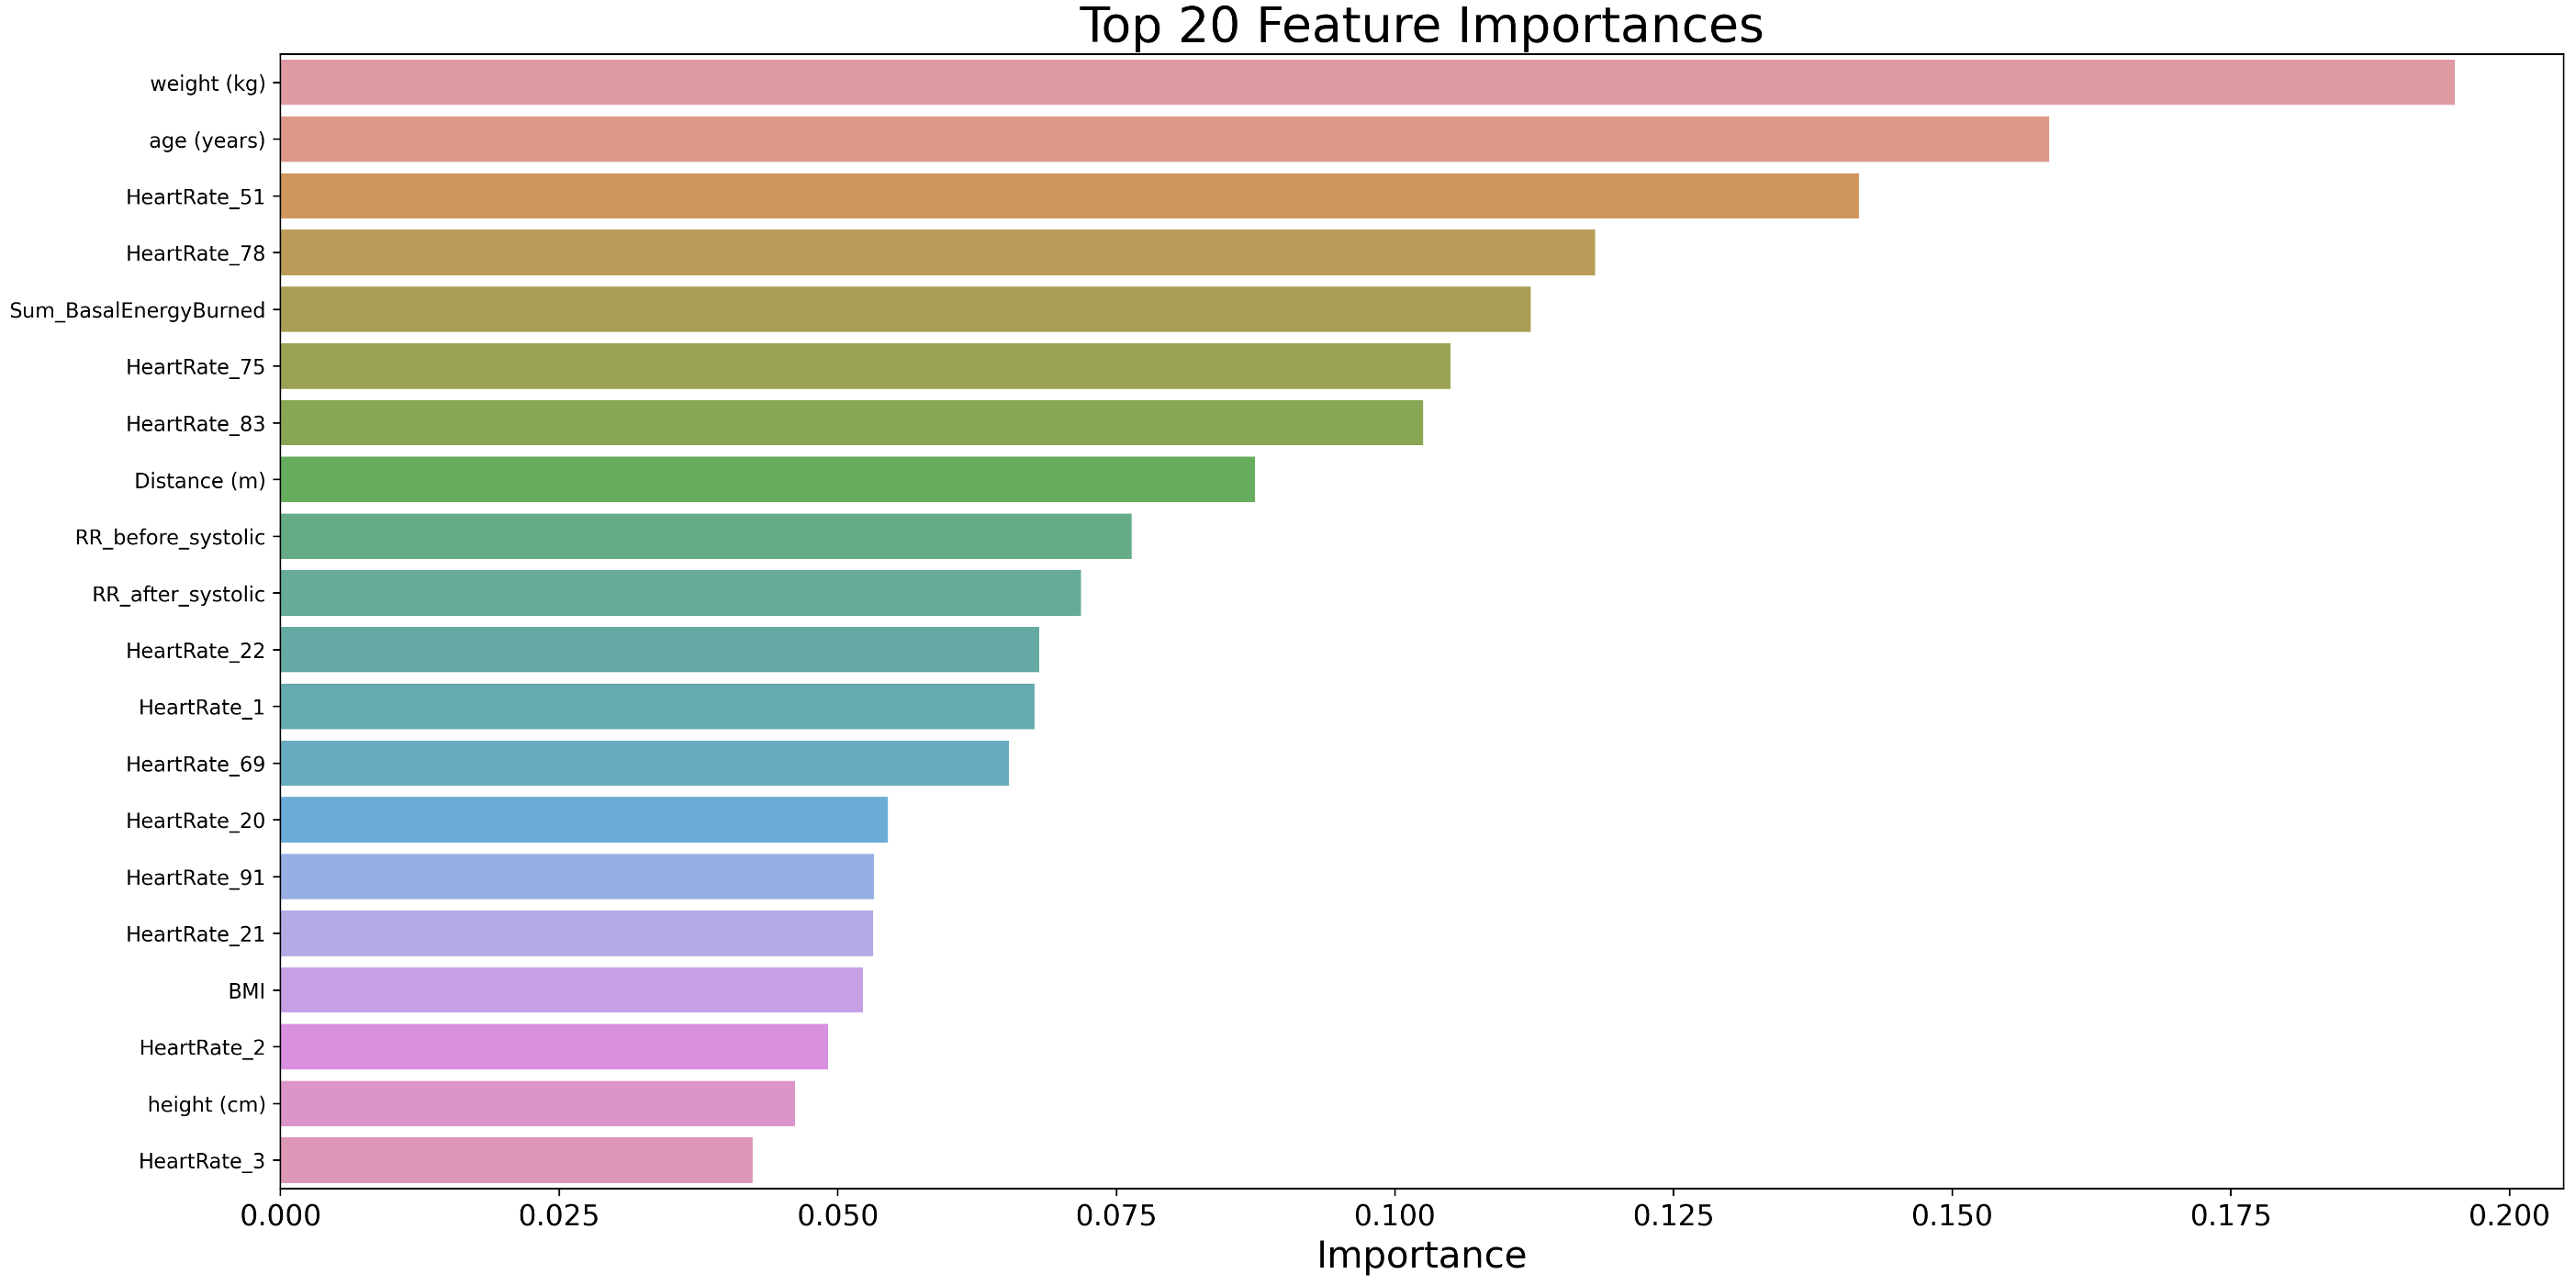
\includegraphics[width=1.0\textwidth]{Master Thesis/Plots/Top_20_Importance_activeEnergy2.png}
        \caption{Feature importance for active energy burned prediction using ridge regression with all given features}
    \label{fig:featureimportanceRRallact}
\end{figure}
\FloatBarrier

Figure ~\ref{fig:featureimportanceRRallact} identifies the top 20 features that the model relies on for predicting active energy burned. The feature weight (kg) emerges as the most critical feature, indicating its significant influence on the model's predictions. The feature age (years) is another key factor, reflecting the impact of age-related metabolic changes on energy expenditure. Various heart rate measurements also play a crucial role, underscoring the importance of the Apple Watch Ultra data in predicting active energy expenditure. Additionally, the basal energy burned feature is highlighted, indicating its strong correlation with active energy burned which is measured by the watch as well. The distance covered by subjects is also a notable predictor, emphasizing the relationship between physical activity and calorie expenditure. Blood pressure measurements before and after the exercise session further contribute to the model's predictions, suggesting the relevance of cardiovascular health metrics.

Continuing our analysis, we focused on predicting basal energy burned, which represents the calories expended at rest to maintain vital bodily functions. The following results detail the model's performance in predicting basal energy burned:

\begin{table}[H]
\begin{longtable}{|>{\raggedright}p{4cm}|>{\raggedright\arraybackslash}p{10cm}|}
\hline
\textbf{metric} & \textbf{value} \\
\hline
\endfirsthead
\hline
\textbf{metric} & \textbf{value} \\
\hline
\endhead
\hline
\endfoot
MSE & 95.17 \\
\hline
RMSE & 9.76 \\
\hline
R\textsuperscript{2} score & 0.21 \\
\hline
CV Scores &
\begin{minipage}[t]{10cm}
[0.23, \ 0.43, \ -0.14, \ -1.04, \ -0.07]
\end{minipage}
\\
\hline
mean CV score & -0.12 \\
\hline
\end{longtable}
\caption{Basal energy burned prediction results with ridge regression based on all measured values}
\label{tab:RRcbasalaloriesallfeatures}
\end{table}

The evaluation of the MSE yielded a value of 95.17, indicating a substantial gap between the predicted and actual basal energy burned values. The RMSE of 9.76 further supports this finding, reflecting the average magnitude of error in the same units as the target variable. These errors suggest that the model's predictions are not highly accurate.

An R\textsuperscript{2} score of 0.21 indicates that only 21\% of the variance in basal energy burned is explained by the features in the model, pointing to a relatively weak explanatory power. This low R\textsuperscript{2} score suggests that there are other factors affecting basal energy burned that are not captured by the model.

The CV scores, ranging from -1.04 to 0.43, reveal variability in the model's performance across different subsets of the data. The presence of negative CV scores for some folds indicates that, in certain cases, the model performs worse than a simple baseline model. The mean CV score of -0.12 further underscores the inconsistency and potential overfitting of the model to specific subsets of the data.

To visualize the significance of the various features, we will present a plot of the top 20 most important features for predicting basal energy burned, providing a clearer understanding of their impact on the model's performance:

\FloatBarrier
\begin{figure}[h!]
    \centering
    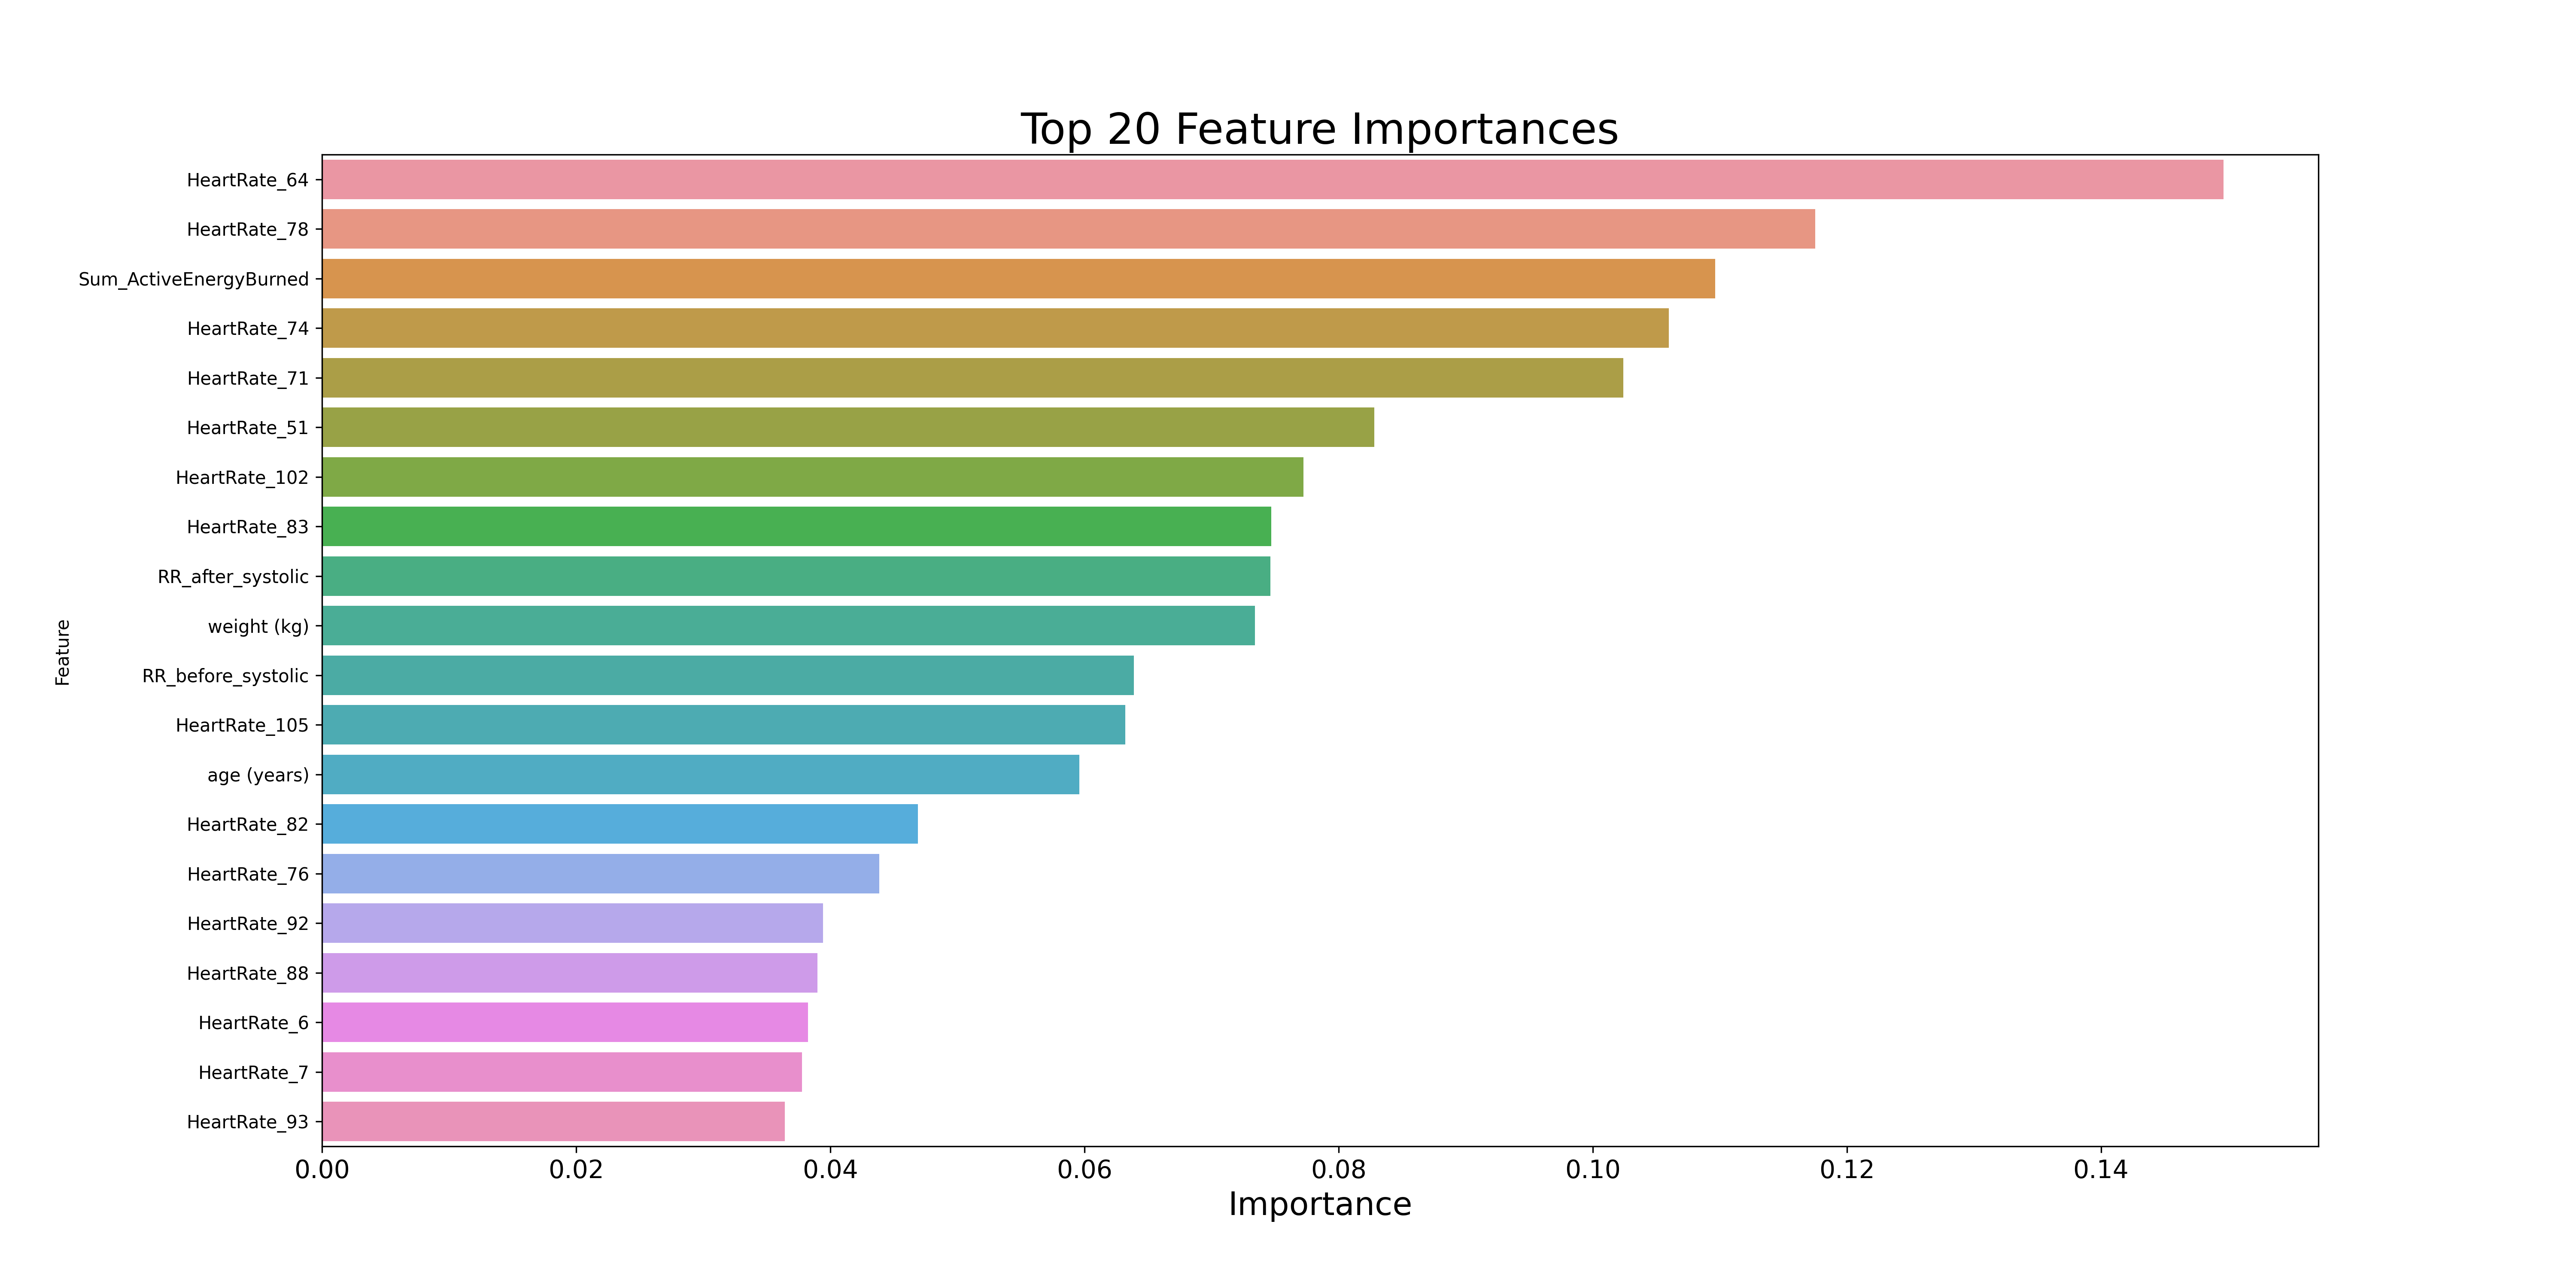
\includegraphics[width=1.0\textwidth]{Master Thesis/Plots/Top_20_Importance_basalEnergy.png}
      \caption{Feature importance for basal energy burned prediction using ridge regression with all given features}
    \label{fig:featureimportanceRRallbas}
\end{figure}
\FloatBarrier

Figure ~\ref{fig:featureimportanceRRallbas} highlights the top 20 features utilized by the model for predicting basal energy burned. Heart rate measurements dominate the list, with 'HeartRate\_64', 'HeartRate\_78', and 'Sum\_ActiveEnergyBurned' being the most influential features. This underscores the critical role of heart rate data in estimating basal energy expenditure. Additional heart rate values, both systolic and diastolic blood pressure measurements, and weight are also significant contributors. The diversity of important features suggests that basal energy burned is influenced by a combination of cardiovascular metrics, body measurements, and overall physical activity.

In summary, while the model demonstrates some capacity to predict basal energy burned, its limited accuracy highlights the need for further refinement and possibly additional features to improve performance.

\subsection{Neural Networks}

We decided to use our new dataset, which has many heart rate measurements and other, not Apple Watch Ultra recorded data, to try NNs again. We hope that these different and additional features will lead to better results. We used all received data in this subsection.

The NN we used has several dense and dropout layers.

The architecture includes:
\begin{itemize}
    \item A dense layer with 256 neurons, ReLU activation, and L2 regularization (0.01)
    \item A dropout layer with a 40\% rate 
    \item Another dense layer with 128 neurons, ReLU activation, and L2 regularization (0.01)
    \item A dropout layer with a 30\% rate
    \item A dense layer with 64 neurons, ReLU activation, and L2 regularization (0.01)
    \item An output layer with 1 neuron
\end{itemize}

The model was compiled using the Adam optimizer and the MSE loss function. Training was conducted for 3000 epochs with a batch size of 32. 

With all these settings we have achieved the following results:

\newpage
\begin{table}[H]
\begin{longtable}{|c|c|c|c|c|}
\hline
\textbf{feature} & \textbf{metric} & \textbf{PCA (n=10)} & \textbf{PCA (n=15)} & \textbf{PCA (n=20)} \\
\hline
\multirow{3}{*}{weight (kg)} & R\textsuperscript{2} & & -15.75 & \\
& MSE & & 13.50 & \\
& RMSE & & \textbf{3.67} & \\
\hline
\multirow{3}{*}{height (cm)} & R\textsuperscript{2} & & -56.58 & \\
& MSE & & 53.39 & \\
& RMSE & & \textbf{7.31} & \\
\hline
\multirow{3}{*}{BMI} & R\textsuperscript{2} & & -1.48 & \\
& MSE & & 0.57 & \\
& RMSE & & \textbf{0.75} & \\
\hline
\multirow{3}{*}{age (years)} & R\textsuperscript{2} & -314.44 & -317.00 & -335.47 \\
& MSE & 311.99 & 314.60 & 333.02 \\
& RMSE & \textbf{17.66} & \textbf{17.74} & \textbf{18.25} \\
\hline
\multirow{3}{*}{leg length (cm)} & R\textsuperscript{2} & -47.17 & -47.59 & \\
& MSE & 44.85 & 45.30 & \\
& RMSE & \textbf{6.70} & \textbf{6.73} & \\
\hline
\multirow{3}{*}{real distance (km)} & R\textsuperscript{2} & & -0.006 & \\
& MSE & & 0.002 & \\
& RMSE & & \textbf{0.047} & \\
\hline
\multirow{3}{*}{BMI over 25} & R\textsuperscript{2} & & -0.03 & \\
& MSE & & 0.01 & \\
& RMSE & & \textbf{0.11} & \\
\hline
\multirow{3}{*}{subject/patient} & R\textsuperscript{2} & & -0.06 & -0.04 \\
& MSE & & 0.04 & 0.02 \\
& RMSE & & \textbf{0.20} & \textbf{0.15} \\
\hline
\end{longtable}
\caption{Comparison of performance between NNs with different PCA setting for various prediction tasks using all features}
\label{tab:PCAdiffallfeatures}
\end{table}

The results for the NN models with different PCA configurations shows mixed performance. Most features have negative R\textsuperscript{2} values, indicating that the models perform worse than a simple mean prediction. This suggests that the models fail to explain the variability of the target variables effectively. Despite the poor R\textsuperscript{2} values, the RMSE values are relatively reasonable. For instance, the RMSE for predicting real distance is 0.047, indicating an average prediction error of 47 meters. However, this may be misleading because the walking distances of most participants are similar, which reduces variability and artificially improves RMSE.

In summary, the negative R\textsuperscript{2} values highlight the poor performance of the models in predicting the target variables, suggesting that the models are not capturing the underlying patterns effectively. While the RMSE values appear reasonable, they might not fully reflect the model's predictive power due to low variability in the dataset. To address these issues, further refinement is necessary to improve the model performance.

\newpage
To enhance the results, we developed a new NN model with a reduced number of PCA components and an optimized architecture tailored for binary classification problems. We first did the subject or patient prediction with all the given data and all features but without the weight. We made adjustments to the loss function and activation function of the output layer and included a validation split to monitor performance. The results are detailed below:

\begin{table}[H]
\begin{longtable}{|>{\raggedright}p{4cm}|>{\raggedright\arraybackslash}p{10cm}|}
\hline
\textbf{metric} & \textbf{value} \\
\hline
\endfirsthead
\hline
\textbf{metric} & \textbf{value} \\
\hline
\endhead
\hline
\endfoot
NN R\textsuperscript{2} on test set (accuracy) & 1.0 \\
\hline
MSE on test set & 0.0 \\
\hline
RMSE on test set & 0.0 \\
\hline
\end{longtable}
\caption{Performance of NN after loss function adjustment using all features for subject or patient prediction}
\label{tab:PCAdiffallfeatures}
\end{table}

The NN achieved an R\textsuperscript{2} value of 1.0 on the test set, indicating perfect predictive performance. Both the MSE and RMSE are 0.0, which further supports the model's accuracy in making predictions. These values suggest that the model is highly precise and has no error in its predictions of a subject or patient for the test set.

The following plots illustrate the accuracy and loss during the training process, offering additional insights into the model's learning dynamics and potential areas for further optimization:

\FloatBarrier
\begin{figure}[h!]
    \centering
    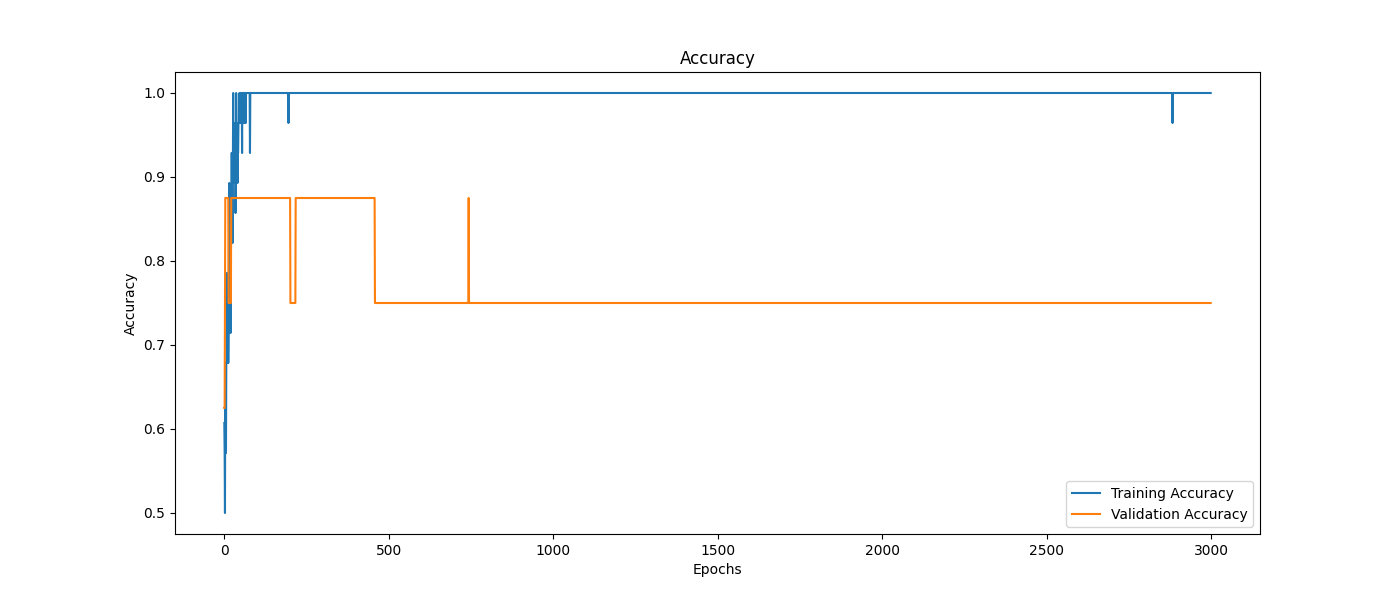
\includegraphics[width=1.0\textwidth]{Master Thesis/Plots/DL_all_Acc.png}
    \caption{Accuracy of deep learning model with extended dataset for subject or patient prediction}
\label{figure:modelaccNNalldata}
\end{figure}
\FloatBarrier

\FloatBarrier
\begin{figure}[h!]
\centering
    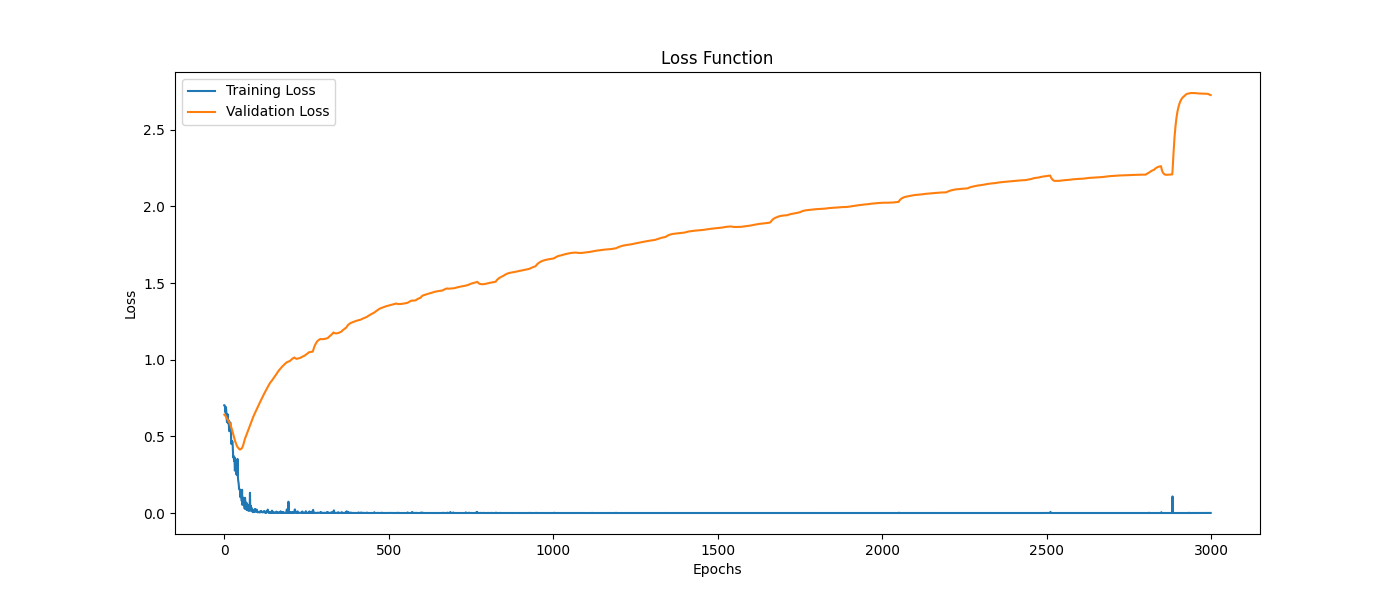
\includegraphics[width=1.0\textwidth]{Master Thesis/Plots/DL_all_Loss.png}
    \caption{Loss of deep learning model with extended dataset for subject or patient prediction}
\label{figure:modellossNNalldat}
\end{figure}
\FloatBarrier

The accuracy plot (Figure ~\ref{figure:modelaccNNalldata}) depicts the model's performance on the training and validation sets across epochs. The training accuracy exhibits significant fluctuations, indicating instability during the learning process. On the other hand, the validation accuracy remains relatively stable but consistently lower than the training accuracy, suggesting that the model struggles to generalize well to new data.

The loss plot (Figure ~\ref{figure:modellossNNalldat}) shows the progression of the loss function over epochs. The training loss decreases steadily, indicating that the model is learning from the data. However, the validation loss is notably higher and increases over time, reinforcing the indication of overfitting. This suggests that while the model is improving its performance on the training set, it does not perform as well on the validation set.

Before we draw a final conclusion on the performance of NN and other ML methods evaluated in this thesis, we aimed to extend our analysis to include risk prediction. Similar to our previous models, we focused on predicting whether a subject has a BMI over 25, which we had classified as a risk factor. This additional analysis provided further insights into the applicability and effectiveness of our models in predicting health-related risks. We achieved following results:

\begin{table}[H]
\begin{longtable}{|>{\raggedright}p{4cm}|>{\raggedright\arraybackslash}p{10cm}|}
\hline
\textbf{metric} & \textbf{value} \\
\hline
\endfirsthead
\hline
\textbf{metric} & \textbf{value} \\
\hline
\endhead
\hline
\endfoot
NN R\textsuperscript{2} on test set (accuracy) & 0.78 \\
\hline
MSE on test set & 0.23 \\
\hline
RMSE on test set & 0.47 \\
\hline
\end{longtable}
\caption{Performance of NN after loss function adjustment using all features for risk prediction}
\label{tab:PCAdiffallfeaturesrisk}
\end{table}

The R\textsuperscript{2} value of 0.78 indicates that the neural network explains 78\% of the variance in the risk prediction task. This is a strong performance, suggesting that the model is fairly accurate in predicting whether a subject has a BMI over 25.

The MSE of 0.23 reflects the average squared difference between the predicted and actual values. While not perfect, this relatively low MSE indicates that the predictions are generally close to the actual outcomes.

The RMSE of 0.47 further quantifies the model's prediction error, providing a more interpretable metric since it is on the same scale as the original values. An RMSE of 0.47 suggests that the model's predictions deviate from the actual values by an average of 0.47 units.

These metrics demonstrate that the NN performs well in the risk prediction task, with a strong R\textsuperscript{2} value and relatively low MSE and RMSE. However, there is still room for improvement.

The following plots illustrate the NNs performance during the risk prediction task, showing the training and validation loss, as well as accuracy over 3000 epochs:

\FloatBarrier
\begin{figure}[h!]
\centering
    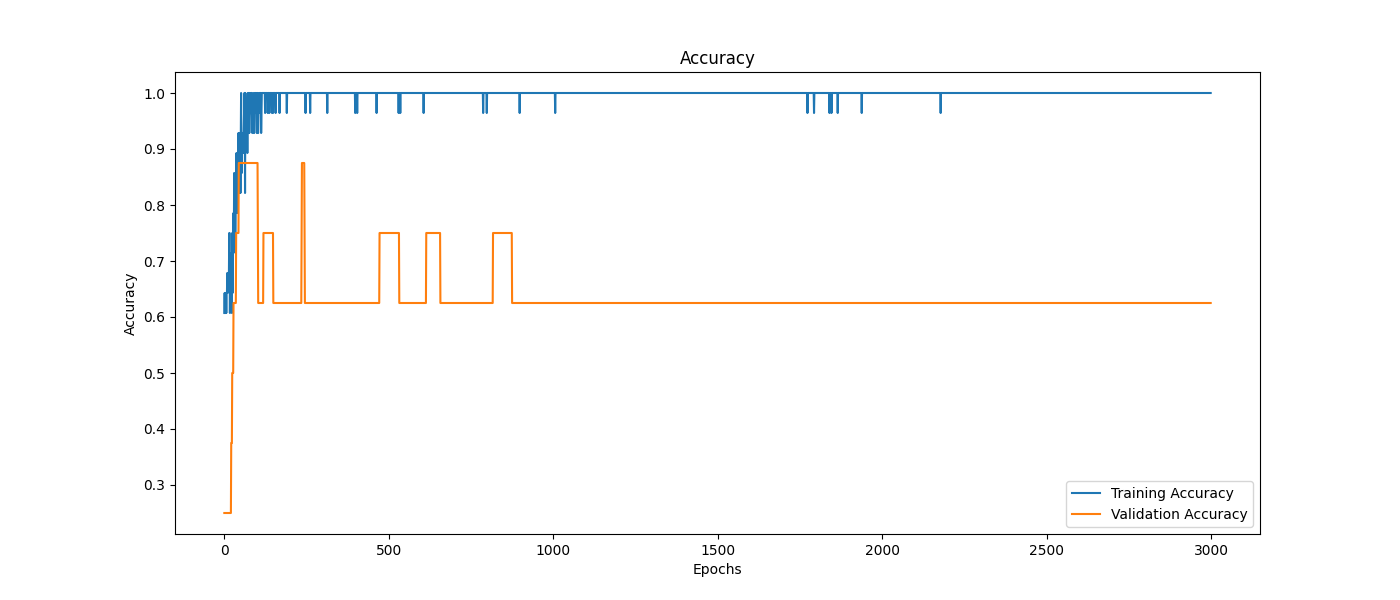
\includegraphics[width=1.0\textwidth]{Master Thesis/Plots/NN_all_risk_loss.png}
    \caption{Accuracy of deep learning model with extended dataset for risk prediction}
\label{figure:modellossNNalldatriskacc}
\end{figure}
\FloatBarrier

\FloatBarrier
\begin{figure}[h!]
    \centering
    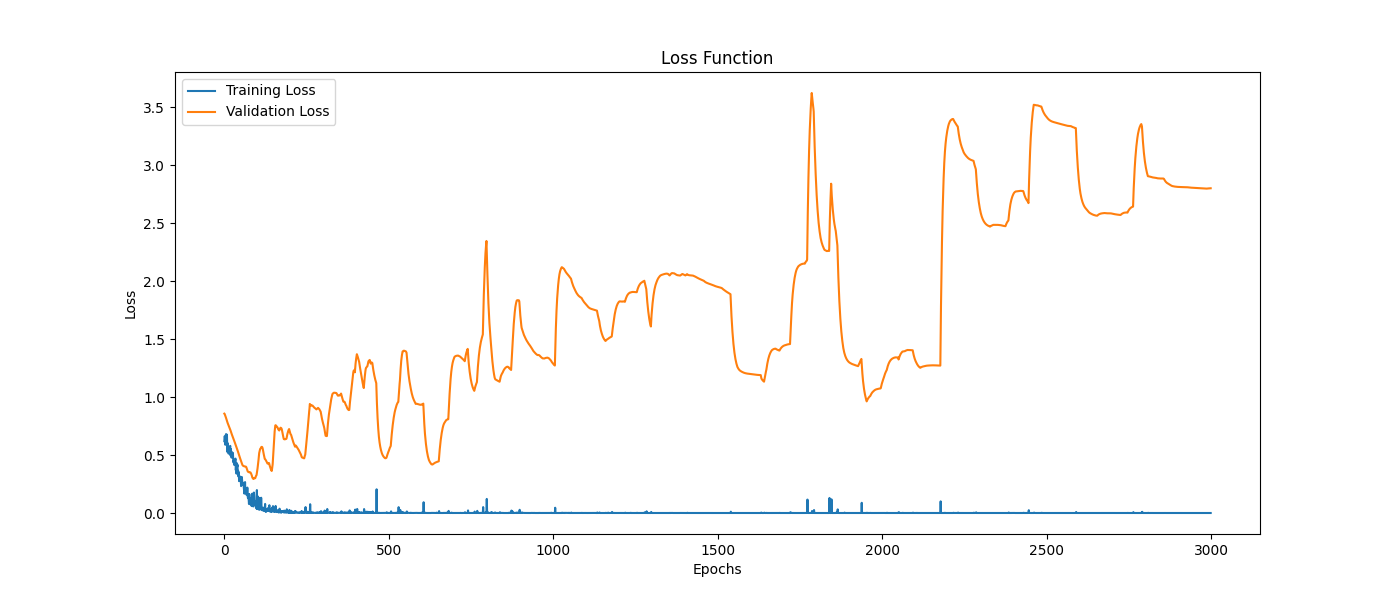
\includegraphics[width=1.0\textwidth]{Master Thesis/Plots/NN_all_risk_acc.png}
    \caption{Loss of deep learning model with extended dataset for risk prediction}
\label{figure:modelaccNNalldatariskloss}
\end{figure}
\FloatBarrier

The accuracy plot (Figure ~\ref{figure:modellossNNalldatriskacc}) demonstrates that the training accuracy (blue line) reaches nearly 1.0 quickly, showing near-perfect performance on the training set. In contrast, the validation accuracy (orange line) remains lower and fluctuates around 0.75, confirming overfitting.

The loss function plot (Figure ~\ref{figure:modelaccNNalldatariskloss}) shows that the training loss (blue line) decreases quickly and stays low, indicating effective learning from the training data. However, the validation loss (orange line) is much higher and fluctuates significantly, indicating overfitting and instability on new data.

These two plots reveal that while the neural network performs well on the training set, it overfits and does not generalize well to the validation set.

In conclusion, while the model shows potential with the comprehensive set of features, it is crucial to address overfitting to ensure robust performance on unseen data. 

Given the nature of our dataset and the specific prediction tasks, we opted not to use unsupervised learning models for this analysis and move directly to the final conclusion, as we do not anticipate better results than those discussed in chapter ~\ref{cha:results}.

\newpage
\section{Summary Table of Chapter Results}
\FloatBarrier
\notsotiny
\begin{longtable}{llrrrrr}
    \caption{Summary of all results in chapter 8 for various models and feature sets} \\
    \toprule
    \textbf{prediction task} & \textbf{features / metrics} & \textbf{precision} & \textbf{recall} & \textbf{f1-score} & \textbf{support} & \textbf{accuracy} \\
    \midrule
    \endfirsthead
    \caption[]{Summary of all results in chapter 8 for various models and feature sets (continued)} \\
    \toprule
    \textbf{prediction task} & \textbf{features} & \textbf{precision} & \textbf{recall} & \textbf{f1-score} & \textbf{support} & \textbf{accuracy} \\
    \midrule
    \endhead
    \bottomrule
    \endfoot
    \multirow{6}{*}{sex prediction (RF)} 
    & age, height, weight, heart rates, blood pressure & & & & & 1.00 \\
    & female & 1.00 & 1.00 & 1.00 & 2.00 & \\
    & male & 1.00 & 1.00 & 1.00 & 4.00 & \\
    & macro avg & 1.00 & 1.00 & 1.00 & 6.00 & \\
    & weighted avg & 1.00 & 1.00 & 1.00 & 6.00 & \\
    \midrule
    \multirow{6}{*}{sex prediction (RF)} 
    & age, height, weight, 100 heart rate values & & & & & 0.78 \\
    & female & 0.71 & 1.00 & 0.83 & 5.0 & \\
    & male & 1.00 & 0.50 & 0.67 & 4.0 & \\
    & macro avg & 0.86 & 0.75 & 0.75 & 9.0 & \\
    & weighted avg & 0.84 & 0.78 & 0.76 & 9.0 & \\
    \midrule
    \multirow{6}{*}{subject/patient prediction (RF)} 
    & age, height, weight, heart rates, blood pressure & & & & & 0.83 \\
    & subject & 0.75 & 1.00 & 0.86 & 3.0 & \\
    & patient & 1.00 & 0.67 & 0.80 & 3.0 & \\
    & macro avg & 0.88 & 0.83 & 0.83 & 6.0 & \\
    & weighted avg & 0.88 & 0.83 & 0.83 & 6.0 & \\
    \midrule
    \multirow{7}{*}{subject/patient prediction (RF)} 
    & age, height, weight, blood pressure and & & & & & 1.00 \\
    & 100 heart rate values & & & & &  \\
    & subject & 1.00 & 1.00 & 1.00 & 6.0 & \\
    & patient & 1.00 & 1.00 & 1.00 & 3.0 & \\
    & macro avg & 1.00 & 1.00 & 1.00 & 9.0 & \\
    & weighted avg & 1.00 & 1.00 & 1.00 & 9.0 & \\
    \midrule
    \multirow{6}{*}{ridge regression (age)} 
    & 100 heart rate values (RMSE) & \multicolumn{4}{c}{14.48} & \\
    & R\textsuperscript{2} on test set & \multicolumn{4}{c}{0.62} & \\
    & MSE & \multicolumn{4}{c}{209.79} & \\
    & mean CV score & \multicolumn{4}{c}{-0.41} & \\
    \midrule
    \multirow{6}{*}{ridge regression (weight)} 
    & 100 heart rate values (RMSE) & \multicolumn{4}{c}{3.57} & \\
    & R\textsuperscript{2} on test set & \multicolumn{4}{c}{0.94} & \\
    & MSE & \multicolumn{4}{c}{12.74} & \\
    & mean CV score & \multicolumn{4}{c}{0.80} & \\
    \midrule
    \multirow{6}{*}{ridge regression (BMI)} 
    & 100 heart rate values and leg length (RMSE) & \multicolumn{4}{c}{2.91} & \\
    & R\textsuperscript{2} on test set & \multicolumn{4}{c}{0.21} & \\
    & MSE & \multicolumn{4}{c}{8.48} & \\
    & mean CV score & \multicolumn{4}{c}{0.63} & \\
    \midrule
    \multirow{6}{*}{ridge regression (height)} 
    & all features (RMSE) & \multicolumn{4}{c}{10.26} & \\
    & R\textsuperscript{2} on test set & \multicolumn{4}{c}{-0.66} & \\
    & MSE & \multicolumn{4}{c}{105.23} & \\
    & mean CV score & \multicolumn{4}{c}{-0.85} & \\
    \bottomrule
\end{longtable}

\newpage
\begin{longtable}{llrr}
    \caption{Summary of all regression results in chapter 8 for various models and feature sets} \\
    \toprule
    \textbf{prediction task} & \textbf{features / metrics} & \textbf{linear regression} & \textbf{ridge regression} \\
    \midrule
    \endfirsthead
    \caption[]{Summary of all regression results in chapter 8 for various models and feature sets (continued)} \\
    \toprule
    \textbf{prediction task} & \textbf{features / metrics} & \textbf{linear regression} & \textbf{ridge regression} \\
    \midrule
    \endhead
    \bottomrule
    \endfoot
    \multirow{3}{*}{weight (kg)} 
     & age, 100 heart rates, blood pressure, energy burned, distance, height & &\\
    & R\textsuperscript{2} & 0.84 &0.99\\
    & MSE & 26.66  &1.21\\
    & RMSE & \textbf{5.16}  &\textbf{1.10}\\
    \hline
    \multirow{3}{*}{height (cm)} 
    & age, 100 heart rates, blood pressure, energy burned, distance, weight & &\\
    & R\textsuperscript{2} &  0.61 &0.98\\
    & MSE & 41.14  &2.27\\
    & RMSE & \textbf{6.41}  &\textbf{1.51}\\
    \hline
    \multirow{3}{*}{BMI}  
    & age, 100 heart rates, blood pressure, energy burned, distance & &\\
    & R\textsuperscript{2} & 0.91 &0.99\\
    & MSE & 0.78 &0.11\\
    & RMSE & \textbf{0.88} &\textbf{0.34}\\
    \hline
    \multirow{3}{*}{age (years)} 
    & 100 heart rates, blood pressure, energy burned, distance, weight, height, BMI & &\\
    & R\textsuperscript{2} & 0.11 & 0.06\\
    & MSE & 449.42 & 476.47\\
    & RMSE & \textbf{21.20} &\textbf{21.83}\\
    \hline
    \multirow{3}{*}{leg length (cm)} 
    & age, 100 heart rates, blood pressure , energy burned, distance, weight, height, BMI & &\\
    & R\textsuperscript{2} & -0.13&0.62\\
    & MSE & 63.35&21.20\\
    & RMSE & \textbf{7.96} &\textbf{4.60}\\
    \hline
    \multirow{3}{*}{real distance (km)} 
    & age, 100 heart rates, blood pressure , energy burned, weight, height, BMI & &\\
    & R\textsuperscript{2} & -1.22&0.72\\
    & MSE & 0.02 &0.00\\
    & RMSE & \textbf{0.13} &\textbf{0.05}\\
    \hline
    \multirow{3}{*}{active energy burned}   
    & age, 100 heart rates, blood pressure , distance, weight, height, BMI & &\\
    & R\textsuperscript{2} & 0.76 \\
    & MSE & 26.47 \\
   & RMSE & 5.14 \\
   & mean CV score & -0.18 \\
    \hline
    \multirow{3}{*}{basal energy burned}   
    & age, 100 heart rates, blood pressure , distance, weight, height, BMI & &\\
    & R\textsuperscript{2} & 0.76 \\
    & MSE & 26.47 \\
   & RMSE & 5.14 \\
   & mean CV score & -0.18 \\
    \bottomrule
\end{longtable}

\normalsize